\documentclass[11pt]{article}
\usepackage[utf8]{inputenc}
\usepackage[T1]{fontenc}
\usepackage[margin=2.2cm]{geometry}
\usepackage{amsmath,amssymb,amsthm}
\usepackage{graphicx}
\usepackage{enumitem}
\usepackage{booktabs}
\usepackage{xcolor}
\usepackage[authoryear,round]{natbib}
\usepackage{hyperref}
\usepackage{lmodern}
\usepackage[font=small,labelfont=bf]{caption}
\newtheorem{proposition}{Proposition}
\graphicspath{{../figures/}{./}}

\title{NetFunrankR: decomposed, exact and calibrated network-proximity enrichment analysis of gene lists}
\author{AKM Azad$^{1,*}$ \and Mohammad Ali Moni$^{2}$}
\date{}

\begin{document}
\maketitle
\noindent{\small $^1$Department of Mathematics and Statistics, College of Science, Imam Mohammad Ibn Saud Islamic University (IMSIU), Riyadh 13318, Saudi Arabia. $^2$Artificial Intelligence \& Data Science, School of Health and Rehabilitation Sciences, The University of Queensland, St Lucia, QLD 4072, Australia. $^*$kazad@imamu.edu.sa}

\begin{abstract}
\noindent\textbf{Motivation:} Over-representation analysis (ORA) only uses genes shared between a query list and a pathway and assumes that every gene is equally likely to be selected, although disease-gene lists are enriched for highly connected, well-studied proteins and pathway annotations are incomplete. Network proximity in the protein interaction network can capture associations that annotation overlap misses, but existing proximity-based approaches mix overlap with network evidence, rely on permutation $z$-scores, and use interactomes that partly encode the annotations being tested.

\noindent\textbf{Results:} We present NetFunrankR, which decomposes the proximity of a gene list to a pathway into a degree-aware overlap test and beyond-overlap tests of the non-member genes (linker count and distance), conditional on the overlap. Under the degree-preserving null of network medicine, all null distributions are computed exactly by discrete convolution (saddlepoint approximation for long lists) and the components are provably independent, giving a valid combined test without permutations. On random hub-biased gene lists, ORA reported significant pathways for 74--100\% of lists of $\ge$50 genes and network enrichment analysis for 100\% of all lists, whereas NetFunrankR controlled false discoveries in every setting ($\le$5.5\%). When 75--90\% of a pathway's genes were missing from its annotation, NetFunrankR retained 2.6-fold the power of ORA (0.62 vs 0.24). On GWAS gene lists for 25 diseases it improved MalaCards phenotype relevance over ORA in 21 diseases (74.4\% vs 59.1\% of optimum), outperformed propagation- and permutation-proximity methods, and doubled the number of disease-relevant significant pathways. On 42 expression datasets of the GSEABenchmarkeR compendium it ranked phenotype-relevant pathways better than ORA, PADOG, GSEA, CAMERA and SAFE while declaring a moderate number of pathways significant. The analysis runs in seconds on a laptop and uses a STRING interactome rebuilt without database- and text-mining-derived edges.

\noindent\textbf{Availability:} R/Bioconductor package with an interactive dashboard, and all benchmark code: \url{https://github.com/Akmazad/NetFunrankR} (MIT licence).
\end{abstract}

\section{Introduction}
Functional enrichment analysis is the default first step in interpreting gene lists produced by genetic association studies, differential-expression experiments or curated disease resources. The most widely used approach, over-representation analysis (ORA), asks whether the query list shares more genes with a pathway than expected under a hypergeometric model \citep{Huang2009}. ORA has three well-documented limitations. First, it only uses \emph{shared} genes: a query gene that is not annotated to a pathway contributes nothing, even if it interacts directly with the pathway's core members. Pathway annotations are, however, incomplete and strongly biased towards well-studied genes \citep{Haynes2018}, and genes implicated by genome-wide association studies (GWAS) frequently act on pathways through interaction partners rather than as annotated members \citep{Barabasi2011,Cowen2017}. Second, the hypergeometric null assumes that every gene is equally likely to be selected and annotated. Highly connected, well-studied proteins are over-represented both among disease genes and among pathway members, which inflates ORA's false-positive rate \citep{Timmons2015,Haynes2018}; an analogous selection bias (gene length in RNA-seq) motivated GOseq \citep{Young2010}. Third, results depend strongly on analysis choices and are often reported without calibration \citep{Wijesooriya2022}.

Network-based enrichment methods use a protein--protein interaction (PPI) network to recover the information that ORA discards. Network enrichment analysis (NEA) and its successors BinoX and ANUBIX count edges between the query and a pathway \citep{Alexeyenko2012,Ogris2017,CastresanaAguirre2020}; EnrichNet and propagation-based methods diffuse the query over the network \citep{Glaab2012,Cowen2017}; pathfindR searches for active subnetworks before running ORA \citep{Ulgen2019}; and topology-based methods such as SPIA use the internal wiring of pathways rather than a genome-wide interactome \citep{Ma2019}. In network medicine, the shortest-path \emph{proximity} of two gene modules, assessed against a degree-preserving random model, has been the workhorse for relating diseases to each other and to drug targets \citep{Menche2015,Guney2016,MorselliGysi2021}. Applying proximity to pathways is natural, but existing implementations, including an earlier, unpublished implementation of our own, share three problems that limit their adoption for enrichment analysis: (i) the proximity score mixes overlap with network evidence, because shared genes have distance zero, so it is unclear whether a network method finds anything that ORA does not; (ii) significance is obtained from a limited number of permutations summarised by a normal approximation, which is slow, has limited resolution in the tail where multiple-testing thresholds lie, and is not guaranteed to be calibrated; and (iii) the interactome itself often contains edges derived from pathway databases (e.g.\ the curated-database channel of STRING), making network proximity to a pathway partly circular.

Here we present NetFunrankR, which addresses all three problems with a single, statistically explicit construction. Our contributions are:
\begin{enumerate}[leftmargin=*,itemsep=2pt]
\item \textbf{A decomposition of network proximity into two independent tests.} The closest-distance proximity of a query to a gene set is split into a degree-aware \emph{overlap} test and \emph{beyond-overlap} tests that evaluate only the non-member query genes---the number of query genes that interact directly with the pathway (linker genes) and their distance to it---conditionally on the membership pattern. We show that the two p-values are independent under the null, so that they can be combined exactly by Fisher's method and each enriched pathway can be attributed to overlap, network proximity or both (Proposition~\ref{prop:indep}).
\item \textbf{Exact, permutation-free degree-preserving null distributions.} Under the standard degree-binned null of network medicine, all three statistics are sums of independent discrete variables whose distributions we compute exactly by convolution (and by a saddlepoint approximation for long lists). This removes the permutation step, gives accurate p-values far into the tail, and reduces run time from hours to seconds.
\item \textbf{A degree-aware overlap test} that corrects the hub bias of the hypergeometric test, and a \textbf{non-circular interactome} (STRING v12 recombined without database and text-mining evidence).
\item \textbf{A comprehensive, multi-scenario validation} against ORA, nine established expression-based methods and four network-based methods: type-I error calibration under realistic hub-biased null lists, power under controlled annotation incompleteness, the GSEABenchmarkeR compendium of 42 expression datasets \citep{Geistlinger2021}, GWAS gene lists for 25 diseases with three independent gold standards including a temporal (prospective) validation, robustness to interactome choice and perturbation, and a COPD case study.
\end{enumerate}

% =====================================================================
% NetFunrankR -- Methods
% Requires: amsmath, amssymb, amsthm (for the proposition), natbib
% =====================================================================
\section{Methods}\label{sec:methods}

\subsection{Overview}
NetFunrankR tests whether a query gene list $X$ (e.g.\ disease genes, GWAS loci or differentially expressed genes) is \emph{closer} to a gene set $Y$ (pathway or functional term) in a protein--protein interaction (PPI) network than expected for degree-matched random genes, and decomposes this proximity into two components with distinct biological meaning: (i) \emph{direct membership}, i.e.\ query genes that are annotated to $Y$ (the information used by over-representation analysis, ORA), and (ii) \emph{network proximity beyond overlap}, i.e.\ query genes that are not annotated to $Y$ but lie closer to its members than expected. Both components are tested against exact, permutation-free, degree-preserving null distributions, and combined into a single enrichment p-value (Figure~\ref{fig:schematic}).

\subsection{Interactome}\label{sec:interactome}
Human protein associations were obtained from STRING v12.0 \citep{Szklarczyk2023} (\texttt{9606.protein.links.detailed.v12.0}) and mapped to HGNC symbols through the STRING protein annotation file. STRING's published combined score integrates seven evidence channels, two of which---\emph{curated databases} (which import KEGG, Reactome and other pathway resources) and \emph{text mining}---are partly derived from the very annotations that enrichment analysis tests. Using them would make network proximity to a pathway partly circular. We therefore recomputed the combined score from the remaining channels $\mathcal{C} = \{$neighbourhood, gene fusion, co-occurrence, co-expression, experiments$\}$ using STRING's own integration rule \citep{vonMering2005}:
\begin{equation}
s^{\mathrm{noKB}} = s^{*} + p_0\,(1 - s^{*}),\qquad
s^{*} = 1 - \prod_{c \in \mathcal{C}} \left(1 - \max\!\left\{\frac{s_c - p_0}{1 - p_0},\, 0\right\}\right),
\label{eq:string}
\end{equation}
where $s_c \in [0,1]$ is the channel score and $p_0 = 0.041$ the STRING prior. Unless stated otherwise, edges with $s^{\mathrm{noKB}} \ge 0.4$ were retained (240,307 edges among 16,024 proteins in the largest connected component, LCC), a network of the same size as the conventional full-evidence STRING network at $s \ge 0.7$. The LCC of the simple undirected graph $G = (V, E)$ was used throughout, so that all shortest-path distances are finite. Sensitivity analyses used $s^{\mathrm{noKB}} \ge 0.7$ and the full-evidence score $s \ge 0.7$ (Section~\ref{sec:robust}).

\subsection{Notation and proximity statistic}
Let $d(u, v)$ denote the shortest-path (hop) distance in $G$ and, for a gene set $Y \subseteq V$,
\begin{equation}
d_Y(v) = \min_{y \in Y} d(v, y), \qquad v \in V,
\end{equation}
the distance from node $v$ to the closest member of $Y$; $d_Y(v) = 0$ if and only if $v \in Y$. For a query $X = \{x_1, \dots, x_n\} \subseteq V$ (query genes absent from the LCC are reported and discarded) we use the \emph{closest-distance} proximity of \citet{Guney2016},
\begin{equation}
d_c(X, Y) = \frac{1}{n}\sum_{i=1}^{n} d_Y(x_i) = \frac{S}{n}, \qquad S = \sum_{i=1}^{n} d_Y(x_i),
\label{eq:dc}
\end{equation}
which was the best-performing proximity measure for drug--disease associations in that study. The vectors $d_Y(\cdot)$ for \emph{all} gene sets of a library are computed simultaneously by a multi-source breadth-first search written as repeated sparse matrix products: with $A$ the adjacency matrix and $F^{(0)}$ the $|V| \times K$ membership indicator of the $K$ gene sets, the frontier at layer $\ell$ is $F^{(\ell)} = \mathbf{1}[A F^{(\ell-1)} > 0] \wedge \neg R^{(\ell-1)}$, where $R$ accumulates visited nodes, and $d_{Y_k}(v) = \ell$ for $F^{(\ell)}_{vk} = 1$. This requires one sparse product per BFS layer (typically $\le 8$) for the whole library, instead of $\sum_k |Y_k|$ single-source searches.

The overlap is $O = |X \cap Y| = \#\{i : d_Y(x_i) = 0\}$ and the \emph{beyond-overlap} distance is $S' = \sum_{i:\, x_i \notin Y} d_Y(x_i)$. Because members contribute zero distance, $S' = S$ numerically; the two statistics differ in their null distributions (below).

\subsection{Degree-preserving null model}
Gene lists from disease studies are strongly enriched for highly connected, well-studied proteins \citep{Barabasi2011,Haynes2018}, and highly connected proteins are both closer to everything and more often annotated to pathways. A valid null must therefore preserve the degree of the query genes. Following \citet{Guney2016}, nodes are sorted by degree and consecutive degree values are pooled into bins $\mathcal{B}_1, \dots, \mathcal{B}_J$ containing at least $b_{\min} = 100$ nodes each. Let $b(i)$ denote the bin of query gene $x_i$. The null hypothesis is
\begin{equation}
H_0:\; x_i \overset{\text{ind.}}{\sim} \mathrm{Uniform}\big(\mathcal{B}_{b(i)} \cap \mathcal{U}\big),\qquad i = 1, \dots, n,
\label{eq:h0}
\end{equation}
i.e.\ each query gene behaves like a random gene of the same degree class, where $\mathcal{U}$ is the background of genes that could have been selected (all network genes by default; the measured genes for expression data). Equation~\eqref{eq:h0} samples with replacement; for bins of $\ge 100$ nodes the difference to sampling without replacement is negligible, which we verified against Monte-Carlo permutation (Supplementary Figure~S1).

For each gene set $Y$ and bin $j$ define the bin-specific distance distribution
\begin{equation}
f_{Y,j}(\delta) = \frac{\#\{v \in \mathcal{B}_j \cap \mathcal{U} : d_Y(v) = \delta\}}{|\mathcal{B}_j \cap \mathcal{U}|}, \qquad \delta = 0, 1, \dots, \delta_{\max},
\end{equation}
whose mass at zero, $\pi_{Y,j} = f_{Y,j}(0)$, is the probability that a random gene of degree class $j$ belongs to $Y$.

\subsection{Exact null distributions by discrete convolution}
Under $H_0$ the summands of $S$ are independent integer-valued variables with probability mass functions $f_{Y, b(i)}$. Hence the null distribution of $S$ is the convolution
\begin{equation}
P_{H_0}(S = s) = \Big(\mathop{\scalebox{1.5}{$\ast$}}_{i=1}^{n} f_{Y,b(i)}\Big)(s) = \Big(\mathop{\scalebox{1.5}{$\ast$}}_{j=1}^{J} f_{Y,j}^{\,\ast m_j}\Big)(s),
\label{eq:conv}
\end{equation}
where $m_j$ is the number of query genes in bin $j$ and $f^{\ast m}$ the $m$-fold self-convolution. The support of $S$ is $\{0, \dots, n\,\delta_{\max}\}$ with $\delta_{\max} \le 10$ in practice, so Equation~\eqref{eq:conv} is evaluated exactly by direct convolution in $O(n^2 \delta_{\max}^2)$ operations. Since all terms are non-negative, direct convolution has no cancellation error and tail probabilities are accurate down to the floating-point underflow limit ($\approx 10^{-300}$), unlike FFT-based convolution or Monte-Carlo permutation, whose resolution is bounded by the number of permutations $B$ ($p \ge 1/(B+1)$). The one-sided \emph{total proximity} p-value is
\begin{equation}
p_{\mathrm{prox}} = P_{H_0}(S \le s_{\mathrm{obs}}).
\end{equation}

\subsection{Decomposition into overlap and beyond-overlap evidence}
\paragraph{Degree-aware overlap test.} Under $H_0$, the membership indicators $I_i = \mathbf{1}[x_i \in Y]$ are independent Bernoulli variables with success probabilities $\pi_{Y, b(i)}$, so $O = \sum_i I_i$ follows a Poisson--binomial distribution, obtained exactly by convolving the $n$ Bernoulli kernels (equivalently, the $J$ binomial distributions $\mathrm{Bin}(m_j, \pi_{Y,j})$):
\begin{equation}
p_{\mathrm{overlap}} = P_{H_0}(O \ge o_{\mathrm{obs}}).
\end{equation}
This test differs from the hypergeometric ORA in one respect: the probability that a query gene hits $Y$ depends on its degree class. When hubs are over-represented both among query genes and among pathway members, the hypergeometric test (which assumes a common probability $|Y|/N$) is anti-conservative, whereas $p_{\mathrm{overlap}}$ is not (Results, Section~\ref{res:calibration}). This mirrors the correction of gene-length bias in RNA-seq ORA by GOseq \citep{Young2010}, with network degree playing the role of gene length.

\paragraph{Beyond-overlap (conditional) proximity test.} Conditionally on the membership pattern $I = (I_1, \dots, I_n)$, each non-member query gene is, under $H_0$, uniform on the non-members of its bin, $\mathcal{B}_{b(i)} \cap \mathcal{U} \setminus Y$, whose distance distribution is the zero-truncated kernel
\begin{equation}
g_{Y,j}(\delta) = \frac{f_{Y,j}(\delta)}{1 - \pi_{Y,j}}, \qquad \delta \ge 1 .
\end{equation}
The conditional null distribution of $S'$ is therefore $\ast_{i: I_i = 0}\, g_{Y, b(i)}$, and
\begin{equation}
p_{\mathrm{beyond}} = P_{H_0}\big(S' \le s'_{\mathrm{obs}} \,\big|\, I\big).
\end{equation}
$p_{\mathrm{beyond}}$ asks whether the query genes that are \emph{not} annotated to $Y$ are nevertheless closer to $Y$ than random non-members of the same degree, i.e.\ whether there is network evidence for an association that annotation-based tests cannot see (because of incomplete annotation, or because the query genes act on the pathway through interaction partners).

\paragraph{Beyond-overlap linker test.} The distance sum $S'$ averages over all non-member query genes; when only a minority of them relate to $Y$ (the typical situation for GWAS loci), the signal is diluted by the many unrelated genes. We therefore also test the number of \emph{linker genes}, non-member query genes that interact directly with a member of $Y$,
\begin{equation}
L = \#\{i : d_Y(x_i) = 1\}.
\end{equation}
Under $H_0$ and conditionally on $I$, each non-member query gene is a linker independently with probability $q_{Y,b(i)} = g_{Y,b(i)}(1)$, so $L$ is Poisson--binomial and
\begin{equation}
p_{\mathrm{linker}} = P_{H_0}\big(L \ge l_{\mathrm{obs}} \,\big|\, I\big)
\end{equation}
is computed exactly (saddlepoint for long lists). $L$ is the beyond-overlap, degree-calibrated analogue of the edge counts used by network enrichment analysis \citep{Alexeyenko2012}: it counts query genes rather than edges, excludes annotated members, and replaces the configuration-model $z$-score with an exact conditional null.

\paragraph{Combination.}
\begin{proposition}\label{prop:indep}
Under $H_0$ (Eq.~\ref{eq:h0}), $p_{\mathrm{overlap}}$ is a function of $I$ only, and the (randomised) conditional p-values $p_{\mathrm{beyond}}$ and $p_{\mathrm{linker}}$ are each uniform on $(0,1)$ conditionally on every value of $I$. Consequently each of them is independent of $p_{\mathrm{overlap}}$ under $H_0$.
\end{proposition}
\begin{proof}[Sketch]
Under $H_0$ the pairs $(I_i, x_i)$ are independent across $i$ and, given $I_i = 0$, $x_i$ is uniform on $\mathcal{B}_{b(i)} \cap \mathcal{U} \setminus Y$. Hence, given $I$, $S'$ and $L$ have exactly the distributions used to compute $p_{\mathrm{beyond}}$ and $p_{\mathrm{linker}}$, so the randomised p-values are $\mathrm{U}(0,1)$ given $I$; their conditional distribution does not depend on $I$, which implies independence from any function of $I$, in particular from $p_{\mathrm{overlap}}$.
\end{proof}
By Proposition~\ref{prop:indep}, Fisher's statistic
\begin{equation}
T = -2\left(\log \tilde p_{\mathrm{overlap}} + \log \tilde p_{\mathrm{linker}}\right) \;\overset{H_0}{\sim}\; \chi^2_4,
\qquad p_{\mathrm{combined}} = P(\chi^2_4 \ge T),
\label{eq:fisher}
\end{equation}
is a valid combined test. NetFunrankR uses the linker test in the combination by default and reports the distance-based combination ($p_{\mathrm{beyond}}$ in place of $p_{\mathrm{linker}}$) as an alternative. This default was chosen after comparing both variants on the GWAS benchmark (Section~\ref{res:gwas}); the expression benchmark, the simulations and the case study were not used for this choice, and results for both variants are reported throughout. Because $O$ and $S'$ are discrete, we use mid-p values $\tilde p = P(\cdot\ \text{more extreme}) + \tfrac12 P(\cdot\ \text{equal})$, which make Fisher's combination of discrete p-values approximately exact rather than conservative \citep{Lancaster1961,Hwang2001}. In contrast to an ad hoc combination of ORA and proximity scores, the decomposition separates the two sources of evidence into independent tests, so that each enriched gene set can be attributed to \emph{overlap only}, \emph{network only}, \emph{both}, or neither component alone (\emph{joint}).

The symmetric module-to-module proximity $d_{XY}$ \citep{Menche2015} and the closest-distance proximity of \citet{Guney2016} are related approaches: both use shortest-path distances with a Monte-Carlo degree-binned null summarised by a $z$-score and a normal approximation, $p = \Phi(z)$; the hypergeometric ORA is recovered from $p_{\mathrm{overlap}}$ when all genes fall into a single bin and $n \ll |V|$.

\subsection{Saddlepoint approximation for long query lists}
For query lists with more than $n_{\mathrm{exact}} = 500$ network genes (e.g.\ differential-expression lists), the $O(n^2)$ convolutions are replaced by the second continuity-corrected Lugannani--Rice saddlepoint approximation for lattice variables \citep{Daniels1987}. With cumulant generating function $K(t) = \sum_j m_j \log \sum_\delta f_{Y,j}(\delta)\, e^{t\delta}$, the upper tail is
\begin{equation}
P(S \ge k) \approx 1 - \Phi(\tilde w) - \phi(\tilde w)\left(\frac{1}{\tilde w} - \frac{1}{\tilde u}\right),\quad
K'(\hat t) = k - \tfrac12,\quad
\tilde w = \mathrm{sgn}(\hat t)\sqrt{2\{\hat t (k - \tfrac12) - K(\hat t)\}},\quad
\tilde u = 2\sinh(\hat t/2)\sqrt{K''(\hat t)},
\end{equation}
and lower tails are obtained from the reflected kernels. The same approximation is applied to $O$ and $S'$. Across all KEGG pathways and query sizes of 100--400 genes, saddlepoint and exact p-values differed by at most $0.02$ on the $\log_{10}$ scale (Supplementary Figure~S1).

\subsection{Multiple testing and output}
Each p-value type is adjusted across gene sets with the Benjamini--Hochberg procedure. Gene sets with fewer than 5 (and, for benchmarks, more than 500) members in the network are not tested. For every gene set NetFunrankR reports the observed and expected overlap, observed and expected $d_c$, standardized effect sizes $z = (\mathrm{E}_{H_0}[S] - S)/\mathrm{SD}_{H_0}[S]$ (computed from the bin-wise cumulants), the five p-values ($p_{\mathrm{overlap}}$, $p_{\mathrm{linker}}$, $p_{\mathrm{beyond}}$, $p_{\mathrm{prox}}$, $p_{\mathrm{combined}}$) with their FDRs, the hypergeometric ORA p-value for reference, the evidence class, and the overlapping and linker genes with the observed and expected linker counts.

\subsection{Compared methods}\label{sec:competitors}
For gene-list input we compared NetFunrankR with: (i) \textbf{ORA}, one-sided hypergeometric test with all genes annotated in the library as background \citep{Huang2009}; (ii) \textbf{NEA}, network enrichment analysis counting query--set edges against the configuration-model expectation $\sum_{x} k_x \sum_{y} k_y / 2|E|$ with a $z$-score \citep{Alexeyenko2012}; (iii) \textbf{RWR}, network propagation by random walk with restart (restart probability 0.5) from the query genes, scoring each set by its mean visiting probability, with a degree-binned permutation null (200 permutations), analogous to EnrichNet \citep{Glaab2012} and propagation-based enrichment \citep{Cowen2017}; (iv) \textbf{Proximity-closest}, the closest-distance proximity of \citet{Guney2016} with 1{,}000 degree-binned permutations and normal p-values; and (v) \textbf{Proximity-symmetric}, the symmetric module-to-module distance $d_{XY} = \left(\sum_{x} \min_{y} d(x,y) + \sum_{y} \min_{x} d(x,y)\right)/(|X|+|Y|)$ \citep{Menche2015} with 200 degree-binned permutations and normal p-values (the statistic of an earlier, unpublished implementation of our tool). All network methods used the same interactome. For expression data we additionally ran the nine set-based methods implemented in EnrichmentBrowser \citep{Geistlinger2016}: ORA, CAMERA \citep{Wu2012}, GSVA \citep{Hanzelmann2013}, GlobalTest \citep{Goeman2004}, SAFE \citep{Barry2005}, GSEA \citep{Subramanian2005}, PADOG \citep{Tarca2012}, ROAST \citep{Wu2010} and SAMGS \citep{Dinu2007} (1{,}000 sample permutations for permutation-based methods).

\subsection{Benchmark design}
\paragraph{Type-I error calibration.}\label{sec:calib_methods}
Random query lists of $n \in \{20, 50, 100, 200\}$ genes were drawn from the network either uniformly or with probability proportional to degree (hub-biased lists, mimicking the hub and study bias of real disease-gene lists; \citealp{Haynes2018}); 200 lists per setting. All methods were applied to the 320 KEGG 2021 pathways (Enrichr), and we recorded the nominal false-positive rate at $\alpha = 0.05$ and the fraction of null lists yielding at least one FDR-significant pathway.

\paragraph{Power under incomplete annotation.}
For 100 randomly chosen KEGG pathways with 50--200 network genes, a fraction $h \in \{0, 0.25, 0.5, 0.75, 0.9\}$ of the pathway's genes was removed from the tested annotation, simulating annotation incompleteness. A query of 50 genes contained $k = sn$ genes drawn from the \emph{complete} pathway ($s \in \{0.1, 0.2, 0.4\}$) and $n - k$ random non-pathway genes. We recorded the proportion of simulations in which the target pathway reached FDR $< 0.05$ (power) and its rank. Because the interactome excludes the curated-database and text-mining channels, hidden members cannot be re-identified through edges derived from KEGG itself.

\paragraph{GSEABenchmarkeR (expression data).}
We used the GEO2KEGG compendium of 42 microarray datasets with phenotype-relevance rankings of KEGG pathways derived from MalaCards \citep{Geistlinger2021}. Expression data were summarised to Entrez genes (\texttt{maPreproc}), differential expression was computed with limma using the benchmark's flexible multiple-testing rule (\texttt{runDE}), and KEGG gene sets (5--500 measured genes) were obtained with EnrichmentBrowser. Gene-list methods used the genes with adjusted $p < 0.05$, exactly the input of EnrichmentBrowser's ORA; NetFunrankR used the measured genes as background $\mathcal{U}$. Performance was quantified by the relevance score, i.e.\ the MalaCards-weighted sum of rank percentiles of the relevant pathways expressed as a percentage of the optimal score (\texttt{evalRelevance}, \texttt{compOpt}), the number of significant sets and the runtime.

\paragraph{GWAS gene lists.}
For the diseases with MalaCards relevance rankings, query lists were the genes mapped to genome-wide significant associations ($p \le 5\times10^{-8}$; GWAS Catalog, \citealp{Sollis2023}) of the matching EFO trait (Supplementary Table~S1). Three gold standards were used: (i) MalaCards relevance as above; (ii) the rank of the disease's own KEGG disease pathway (e.g.\ \textit{Alzheimer disease} for Alzheimer's disease GWAS), in the spirit of the target-pathway benchmark of \citet{Tarca2012}; and (iii) a \emph{temporal} validation that does not rely on curated disease--pathway associations: each disease's genes were split at the median date of first report into \emph{early} and \emph{late} genes, methods were applied to the early genes only, and their pathway rankings were evaluated (AUROC, AUPRC) against the pathways over-represented among the late genes (hypergeometric $p < 0.01$, late genes not in the early list). This asks whether a method applied to today's gene list anticipates the pathways implicated by tomorrow's discoveries.

\paragraph{Robustness.}\label{sec:robust}
The GWAS benchmark was repeated with (a) alternative interactomes (STRING noKB $\ge 0.7$, full-evidence STRING $\ge 0.7$), (b) random removal of 10, 25 and 50\% of edges, (c) degree-preserving rewiring of the network (negative control; three replicates each), and (d) minimum degree-bin sizes of 50 and 250. Stability was assessed by drawing 20 random halves of each GWAS list and computing the Jaccard index between the top-20 pathways of the half and of the full list.

\paragraph{Case study.}
The 307 COPD genes of \citet{MorselliGysi2021} (bundled with the package) were analysed against KEGG. Agreement with MalaCards COPD relevance was evaluated for all methods and for random subsets of 6--50 genes, and pathway rankings were compared with CAMERA results on an independent COPD expression dataset (GSE42057, part of GEO2KEGG).

\subsection{Implementation and availability}
NetFunrankR is an R/Bioconductor package (R $\ge 4.4$) with the convolution kernel implemented in C++ (Rcpp) and an interactive Shiny dashboard (\texttt{runNetFunrankRApp()}) that accepts any gene-set library and interactome and can be self-hosted (a Docker recipe is provided). Interactome distances for a library are computed once (2.8\,s for KEGG on a laptop) and reused across queries; a complete KEGG analysis of a 300-gene query takes about 2\,s on one core. The package bundles the STRING v12 networks described above, KEGG, Reactome and WikiPathways libraries, and provides the evidence map, null-distribution and linker-network visualizations used in this paper. All benchmark code is in \texttt{analysis/} of the repository (\url{https://github.com/Akmazad/NetFunrankR}).

\section{Results}

\subsection{Exact null distributions replace permutation testing}
For every gene set, NetFunrankR computes the null distributions of the overlap, linker count and distance statistics exactly (Figure~\ref{fig:schematic}). Exact p-values agreed with 2{,}000 degree-binned Monte-Carlo permutations (Spearman $\rho = 0.9994$ between $\log_{10}$ p-values of the 320 KEGG pathways for the COPD list; all differences within Monte-Carlo error), and the saddlepoint approximation used for long lists differed from the exact values by at most $0.02$ $\log_{10}$ units (Supplementary Figure~S1). Unlike permutation p-values, which cannot fall below $1/(B+1)$, the exact p-values resolve the extreme tail (e.g.\ $p = 1.3\times10^{-7}$ for \textit{Nicotine addiction} in the COPD analysis, where 2{,}000 permutations give $p \ge 5\times10^{-4}$). Removing the permutation step also removes the main computational bottleneck (Supplementary Figure~S2): the original NetFunrankR v1 implementation required 26\,s per pathway for only 100 permutations (2.3\,h for the 320 KEGG pathways), whereas v2 tests all KEGG pathways in 0.5--3.4\,s and all Reactome pathways in 3.4--24\,s for query lists of 10--2{,}000 genes on a single laptop core, after a one-off distance computation per library (2.8\,s for KEGG, 20\,s for Reactome). This is comparable to Proximity-$z$ with 1{,}000 permutations (0.1--20\,s), whose p-values, however, rest on a normal approximation of the permutation $z$-score that is miscalibrated (Section~\ref{res:calibration}).

\subsection{Hub-biased gene lists inflate false discoveries of ORA and published network methods}\label{res:calibration}
We first asked whether each method controls false positives when the query list contains no biological signal (Figure~\ref{fig:calibration}). For uniformly sampled random lists, ORA was conservative (1.6--3.3\% of pathways at $p<0.05$), whereas NEA was strongly anti-conservative (15.6--19.2\%), and 100\% of random lists produced at least one FDR-significant pathway with NEA. Random lists that over-represent highly connected proteins---as disease-gene and GWAS lists do---changed the picture for ORA: its per-pathway false-positive rate rose with list size to 7.5\% ($n = 200$), and the fraction of random lists with at least one FDR-significant pathway reached 26\%, 74\%, 99\% and 100\% for $n = 20$, 50, 100 and 200, respectively. Permutation-based proximity with a normal approximation (Proximity-$z$; NetFunrankR v1 statistic) was mildly anti-conservative (per-pathway rates up to 6.3\% and 6.9\%), yielding spurious FDR-significant pathways for 5--13\% and 9--22\% of random lists. All NetFunrankR v2 tests were calibrated in every setting: per-pathway false-positive rates were at most 5.4\% (combined test: 3.2--4.9\%), and at most 5.5\% of random lists produced any FDR-significant pathway with the combined test. RWR with 200 permutations was calibrated but, owing to its permutation floor, could not produce p-values below $5\times10^{-3}$ (flat segment in Figure~\ref{fig:calibration}a), which made FDR-significant findings practically unreachable (Sections~\ref{res:power}--\ref{res:gwas}). These results show that the degree-preserving null is not a technicality: without it, hub-rich gene lists generate pathway ``enrichments'' by construction.

\subsection{Network proximity recovers pathways with incomplete annotation}\label{res:power}
We next planted pathway signal into random query lists while hiding a growing fraction of the pathway's genes from the tested annotation (Figure~\ref{fig:power}; 100 KEGG pathways, 50-gene lists). With complete annotation all overlap-based tests detected the target pathway when 20\% of the query came from it (power 0.99--1.00), whereas distance-only proximity (Proximity-$z$ 0.81; NetFunrankR total proximity 0.79) and RWR (0.41) were less sensitive. As annotation became incomplete, ORA lost power rapidly (0.54 and 0.24 with 75\% and 90\% of the pathway hidden), while the NetFunrankR combined test retained 0.80 and 0.62, because hidden pathway members were recovered as linker genes. The combined test also ranked the target pathway best among calibrated methods (median rank percentile 1.3\% and 3.5\% at 75\% and 90\% hidden, versus 6.1\% and 15.4\% for ORA). NEA (0.93 and 0.73) and the NetFunrankR v1 statistic (0.77 and 0.49) were also robust, but at the price of the type-I error inflation shown above; NEA ranked the target lower than NetFunrankR in every setting. With strong signal (40\%) every method except RWR exceeded power 0.85 at 90\% hidden annotation, and NetFunrankR reached 0.93 versus 0.58 for ORA. The cost of combining two tests appeared only for the weakest signal (10\%, i.e.\ five pathway genes) with complete annotation, where the combined test had lower power than ORA (0.70 vs 0.90) because the linker component carried no information; with 25\% or more of the annotation missing the two were equivalent.

\subsection{Expression benchmark (GSEABenchmarkeR)}\label{res:gseabench}
On the 42 GEO2KEGG expression datasets (Figure~\ref{fig:gseabench}), gene-list methods applied to the differentially expressed genes ranked MalaCards-relevant pathways at least as well as methods using the full expression data, in line with the original benchmark, in which ORA and PADOG were among the best performers \citep{Geistlinger2021}. NetFunrankR (64.8\% of the optimal relevance score) outperformed ORA (60.4\%; better in 27/42 datasets, paired Wilcoxon $p = 0.006$), PADOG (61.5\%; 29/42, $p = 0.045$), SAFE (58.1\%; $p = 6\times10^{-4}$), GSEA (54.5\%; 35/42, $p = 1.6\times10^{-6}$), CAMERA (53.8\%; $p = 7\times10^{-5}$), GSVA, ROAST, SAMGS and RWR (61.2\%; 35/42, $p = 8\times10^{-5}$), and did not differ significantly from GlobalTest (61.8\%; $p = 0.08$), NEA (64.9\%; $p = 0.79$) or Proximity-$z$ (66.9\%; $p = 0.07$). The degree-aware overlap test alone again improved on the hypergeometric test (28/42 datasets, $p = 0.007$ for the combined versus overlap-only comparison; Figure~\ref{fig:gseabench}a). The number of significant sets distinguished the network methods sharply: NEA and Proximity-$z$ declared a median of 44\% and 74\% of all KEGG pathways significant per dataset---as did GlobalTest (89\%) and SAMGS---whereas NetFunrankR reported a median of 8.1\%, comparable to CAMERA (8.7\%) and GSVA (7.0\%). With long expression-derived lists (median 1{,}845 DE genes), NetFunrankR used the saddlepoint approximation and required a median of 11\,s per dataset, compared with 70\,s for PADOG and 176\,s for GSEA with 1{,}000 sample permutations.

\subsection{GWAS gene lists: three independent gold standards}\label{res:gwas}
Gene lists from GWAS are the setting in which annotation-based enrichment is weakest, because many associated genes are not (yet) annotated to the pathways through which they act. We assembled genome-wide significant gene lists for 25 diseases (15--1{,}387 network genes; Supplementary Table~S1) and evaluated all methods against three gold standards (Figure~\ref{fig:gwas}).

\emph{MalaCards relevance.} All network methods ranked phenotype-relevant pathways higher than ORA (mean relevance 59.1\% of the optimum). The NetFunrankR combined test reached 74.4\%, outperforming ORA in 21 of 25 diseases (paired Wilcoxon $p = 3.2\times10^{-5}$), RWR (69.9\%; 21/25, $p = 2.2\times10^{-5}$), Proximity-$z$ (69.6\%; 20/25, $p = 6.3\times10^{-4}$) and the distance-based combination (71.2\%; 17/25, $p = 0.008$), and performing on par with NEA (75.0\%; $p = 0.56$) and the NetFunrankR v1 statistic (73.0\%; $p = 0.21$)---the two methods with inflated type-I error. Notably, the degree-aware overlap test alone improved on the hypergeometric test (66.3\% vs 59.1\%; 21/25 diseases, $p = 4.2\times10^{-6}$), showing that correcting hub bias also improves the \emph{ranking} of relevant pathways.

\emph{Significant findings.} Because ranking metrics ignore calibration, we also examined what users act on: pathways called at FDR $<0.05$. The combined test reported 1{,}259 significant disease--pathway pairs across 25 diseases, of which 321 were MalaCards-relevant, compared with 148 relevant among 438 for ORA; i.e.\ NetFunrankR more than doubled the number of relevant significant pathways and produced significant results for 22 rather than 19 diseases, at a lower precision (25\% vs 34\%). Since the MalaCards rankings are themselves derived from gene overlap between disease genes and pathways, this precision estimate is expected to favour overlap-based methods. NEA reported 3{,}734 significant pairs, which, given its calibration (Section~\ref{res:calibration}), cannot be interpreted as discoveries.

\emph{Target disease pathway.} For the 21 diseases with a dedicated KEGG disease pathway, the combined test called the target pathway significant (FDR $<0.05$) in 11 diseases, compared with 8 for ORA and 3 for RWR; median target ranks were similar for ORA (7th percentile), the degree-aware overlap test (6th) and the combined test (9th).

\emph{Temporal validation.} When methods were applied only to the genes reported up to each disease's median discovery date, the pathways they prioritised predicted the pathways over-represented among genes discovered later (mean AUROC: NEA 0.795, NetFunrankR 0.767, RWR 0.757, ORA 0.755; 10 diseases). The difference between NetFunrankR and ORA was not significant (6/10 diseases; $p = 0.70$), whereas both distance-only statistics (Proximity-$z$ 0.704; NetFunrankR distance test 0.641) performed worst, confirming that the linker formulation is the better beyond-overlap statistic for sparse genetic signals.

\subsection{Robustness}\label{res:robust}
The GWAS benchmark was repeated under alternative interactomes and perturbations (Figure~\ref{fig:robust}). Removing STRING's curated-database and text-mining channels did not cost performance---it improved it: the combined test reached 74.4\% relevance on the non-circular network versus 71.9\% on the conventional full-evidence network (score $\ge 0.7$) and 71.7\% on the smaller high-confidence non-circular network. Results were insensitive to the degree-bin size (74.2\% for minimum bin sizes of 50 and 250) and to missing interactions (73.9\% and 73.7\% after removing 25\% and 50\% of the edges). As a negative control, degree-preserving rewiring of the interactome, which keeps every protein's degree but destroys biological wiring, reduced the linker test from 70.5\% to 58.4\%---the level of ORA---and the distance test from 64.7\% to 53.2\%, while the overlap component was unaffected. Hence the beyond-overlap evidence reflects the specific topology of the interactome rather than degree artefacts. Finally, results were as stable as ORA under subsampling of the query: the top-20 pathways obtained from random halves of each GWAS list overlapped those from the full list with a mean Jaccard index of 0.44 for the combined test and 0.47 for ORA, compared with 0.40 for Proximity-$z$ and 0.36 for RWR.

\subsection{Case study: COPD}\label{res:copd}
The 307 COPD-associated genes of \citet{MorselliGysi2021} (261 in the network) were tested against 363 KEGG pathways (Figure~\ref{fig:copd}). The combined test identified 24 pathways at FDR $<0.05$: 11 supported mainly by overlap, 7 by both overlap and linker genes, and 6 by network evidence only, compared with 7 pathways for the hypergeometric ORA. The NetFunrankR ranking agreed best with MalaCards COPD relevance (77.9\% of optimum; NEA 73.9\%, ORA 70.0\%, Proximity-$z$ 68.1\%, RWR 66.4\%). It was also the ranking most consistent with an independent \emph{expression} analysis of COPD (CAMERA on peripheral blood transcriptomes, GSE42057; Spearman $\rho = 0.10$ for the combined and $0.14$ for the linker test, versus $0.00$ for ORA), although agreement between genetic and transcriptomic evidence was weak for all methods. The advantage of network evidence was largest for short lists: with random subsets of 6 or 10 COPD genes, ORA recovered only 9.4\% and 8.5\% of the optimal relevance score, whereas NetFunrankR reached 54.9\% and 52.8\%, comparable to the other network methods but with calibrated significance (Figure~\ref{fig:copd}c).

\section{Discussion}
Network proximity is a central concept of network medicine, but its use for functional enrichment has remained ad hoc: proximity scores mix annotation overlap with network evidence, significance rests on a limited number of permutations and a normal approximation, and the interactome may itself encode the pathway annotations being tested. NetFunrankR v2 turns proximity-based enrichment into a statistically explicit procedure. The key observation is that, under the standard degree-preserving null model of network medicine, overlap, distance and linker statistics are sums of independent discrete variables, so their null distributions can be computed exactly. Conditioning on the membership pattern then separates the evidence into an overlap test and beyond-overlap tests that are independent under the null (Proposition~\ref{prop:indep}). This yields (i) a valid combined test, (ii) an attribution of each finding to direct annotation, network context, or both, and (iii) p-values that are exact far into the tail at a fraction of the cost of permutation testing.

Three results stand out from the benchmarks. First, calibration matters more than is commonly appreciated. Random gene lists that merely over-represent highly connected proteins---a property shared by most disease-gene and GWAS lists---made the hypergeometric ORA report FDR-significant pathways for almost every list of 100 genes or more, and NEA did so for every list regardless of composition. A degree-aware overlap test removes this artefact and, perhaps surprisingly, also improves the ranking of phenotype-relevant pathways. Second, network evidence is most valuable exactly where annotation-based enrichment is weakest: for incomplete annotation (simulation), for GWAS gene lists, and for short lists, where ORA recovered less than 10\% of the attainable COPD relevance from 6--10 genes while NetFunrankR recovered more than half. Third, among beyond-overlap statistics the number of linker genes was clearly superior to mean distance for genetic data, consistent with sparse signals in which only a minority of loci relate to a given pathway; the distance statistic, which underlies previous proximity analyses including NetFunrankR v1, was the weakest component.

Several limitations should be noted. The null model treats query genes as independent draws within degree bins; it does not model linkage disequilibrium between GWAS loci, gene length, or co-regulation of differentially expressed genes, which can induce dependence among query genes. Like ORA, NetFunrankR is a competitive test of a gene list and cannot exploit the continuous statistics or sample structure that self-contained expression methods use; on expression data it should therefore be viewed as complementary to methods such as CAMERA or PADOG rather than as a replacement. MalaCards relevance rankings, the gold standard of GSEABenchmarkeR, are partly derived from gene overlap and are incomplete, which favours overlap-based methods and limits the attainable precision of any method that reports pathways supported by network evidence only; the simulations and the temporal validation were designed to complement this. The choice of the linker statistic as the default beyond-overlap test was made on the GWAS benchmark, and we therefore report both variants throughout; the other benchmarks were not used for method selection. Finally, interactome coverage remains biased towards well-studied proteins. Removing the curated-database and text-mining channels of STRING eliminates direct circularity but not this study bias, which the degree-preserving null mitigates but cannot remove entirely.

Beyond pathway enrichment, the same construction applies whenever a gene list is compared with a gene module in a network, for example drug targets versus disease modules \citep{Guney2016} or disease--disease relationships \citep{Menche2015}, where exact, decomposed and calibrated tests could replace permutation $z$-scores.


\section*{Funding}
The authors extend their appreciation to the King Salman Center for Disability Research for funding this work through research group no KSRG-2023-456.

\section*{Data availability}
STRING v12.0, GWAS Catalog (release used: October 2026), GEO2KEGG compendium and MalaCards relevance rankings (GSEABenchmarkeR) are publicly available; processed inputs, result tables and scripts reproducing every figure are provided in the repository (\texttt{analysis/}).

\bibliographystyle{plainnat}
\bibliography{references}

\clearpage
\section*{Figures}

\begin{figure}[h]
\centering
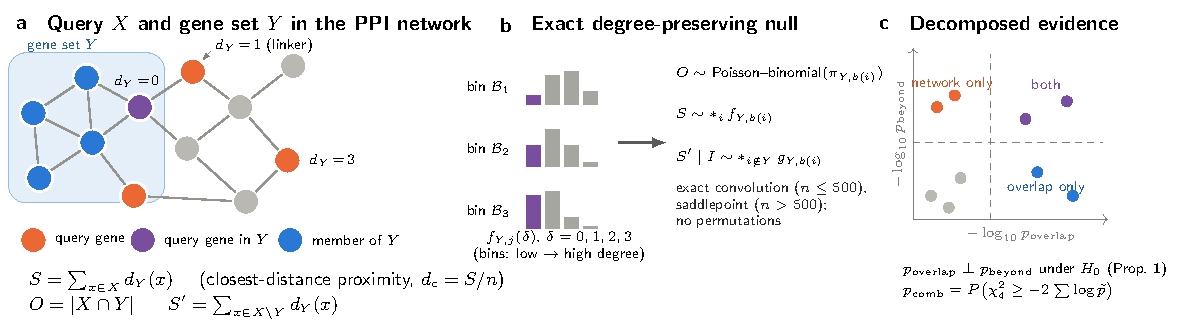
\includegraphics[width=\linewidth]{fig1_schematic.pdf}
\caption{\textbf{NetFunrankR.} \textbf{a} For a query $X$ and gene set $Y$, every query gene contributes its shortest-path distance $d_Y(x)$ to the closest member of $Y$ (0 for members, 1 for linker genes that interact directly with a member). \textbf{b} Under the degree-preserving null, query genes are replaced by random genes of the same degree bin; the bin-specific distance distributions $f_{Y,j}$ yield the exact null distributions of the overlap $O$ (Poisson--binomial), the total distance $S$, and---conditionally on the membership pattern $I$---the linker count and distance of the non-member genes. \textbf{c} The overlap and beyond-overlap p-values are independent under the null (Proposition~\ref{prop:indep}) and are combined with Fisher's method; each pathway is attributed to overlap, network (linker) evidence, or both.}
\label{fig:schematic}
\end{figure}

\begin{figure}[p]
\centering
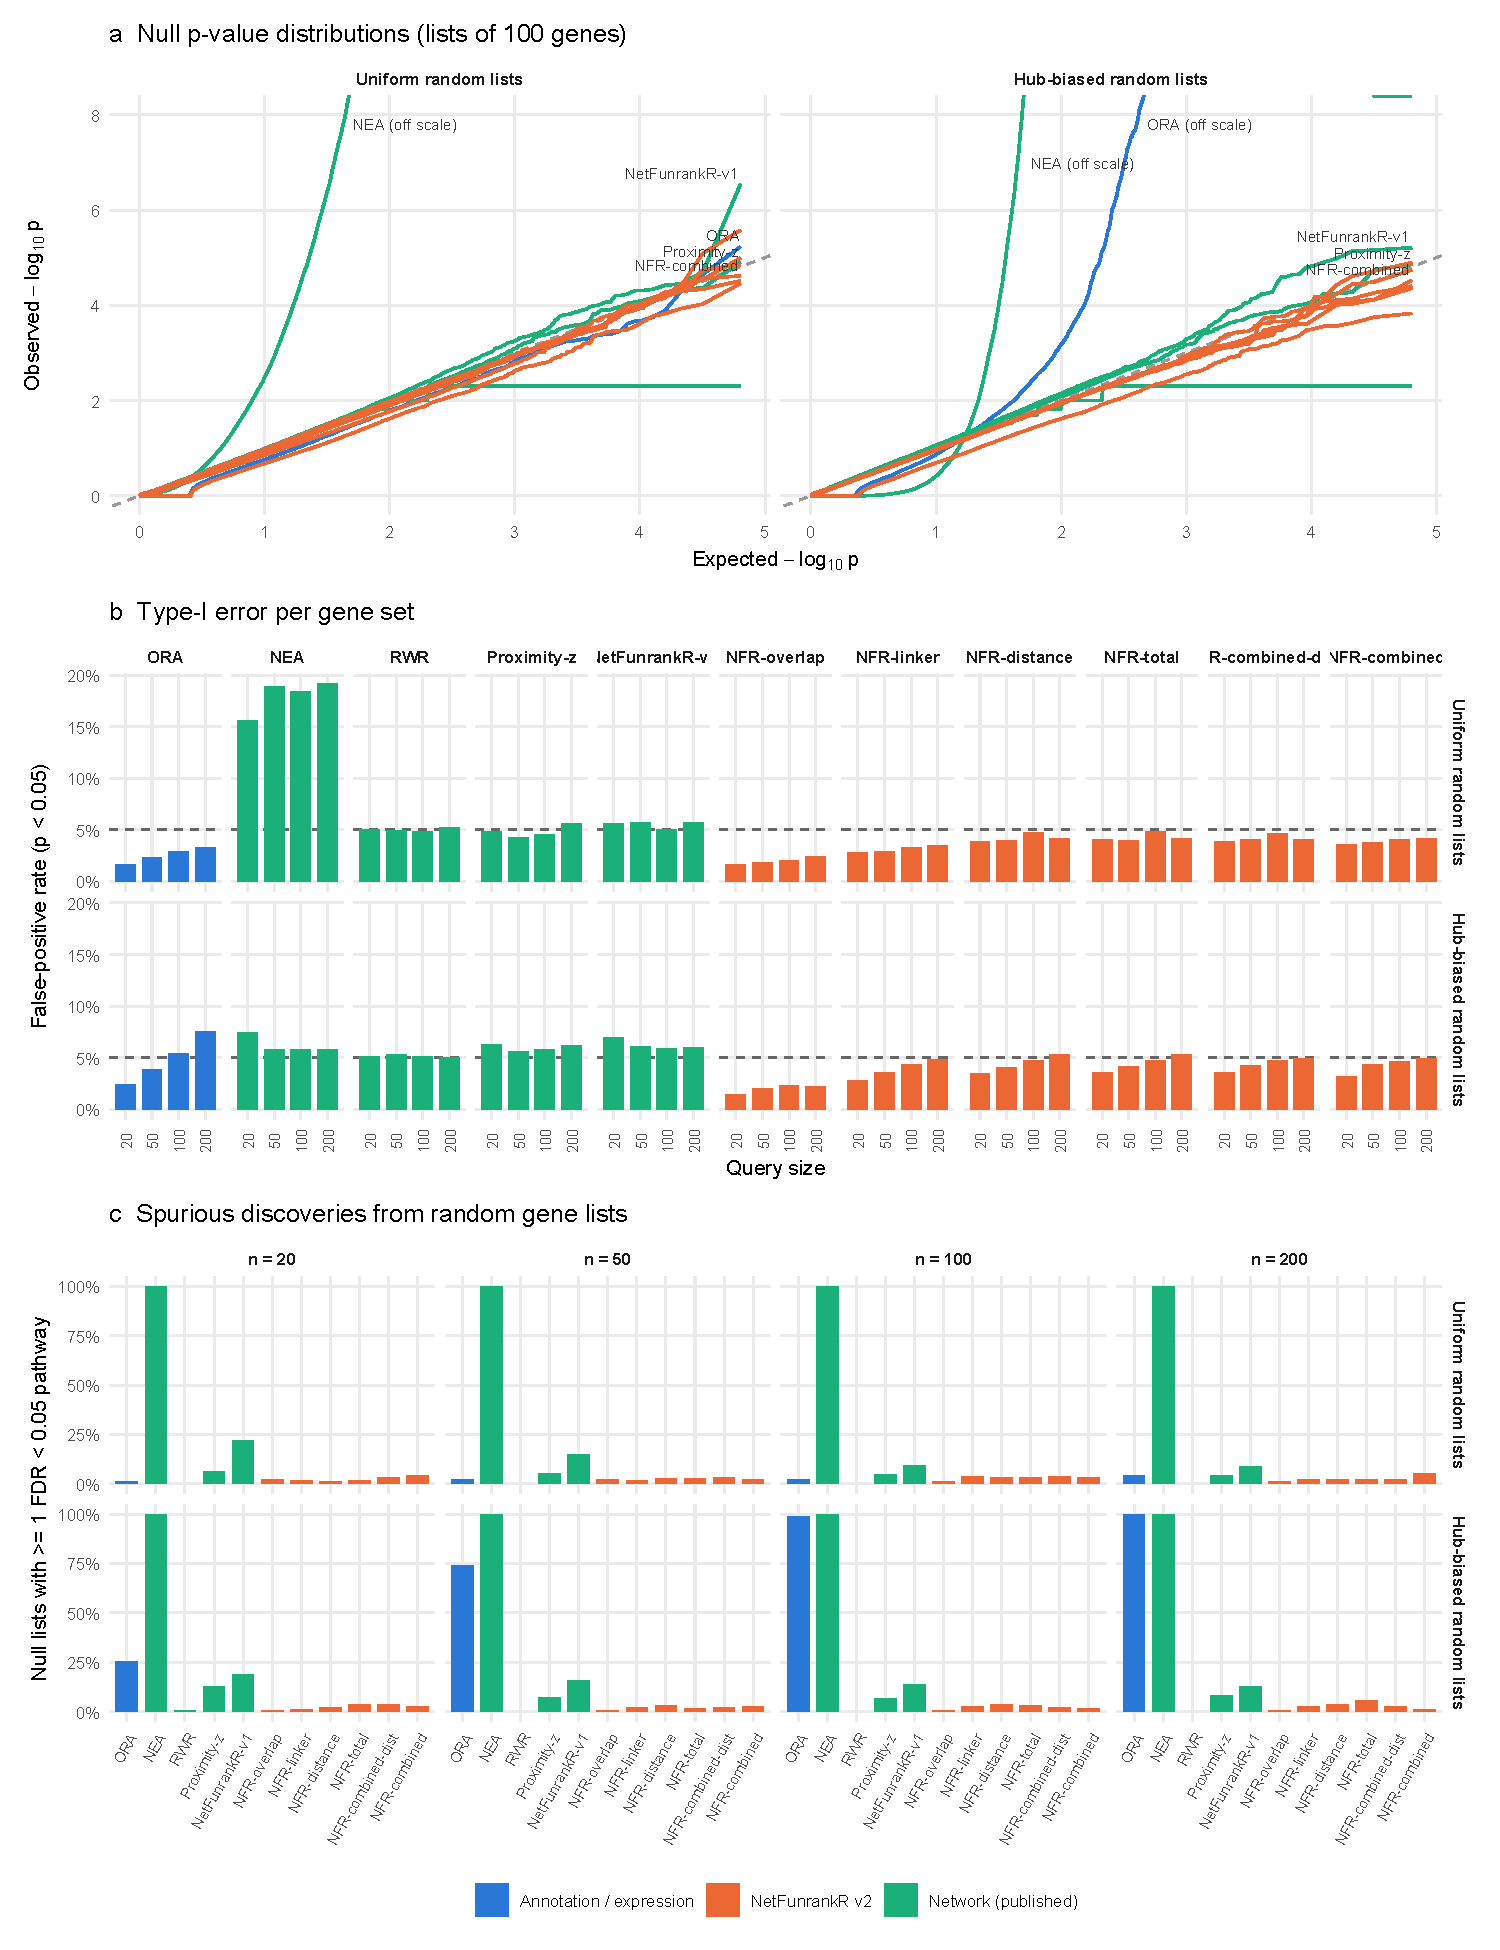
\includegraphics[width=0.93\linewidth]{Fig2_calibration.pdf}
\caption{\textbf{Type-I error under random gene lists.} 200 random lists per setting were drawn uniformly or with probability proportional to degree (hub-biased) and tested against 320 KEGG pathways. \textbf{a} Quantile--quantile plots of pathway p-values (lists of 100 genes; dashed: uniform expectation). \textbf{b} Fraction of pathways with $p < 0.05$ (dashed: nominal 5\%). \textbf{c} Fraction of random lists with at least one pathway at FDR $< 0.05$. RWR p-values are bounded below by its 200 permutations (flat segment in a).}
\label{fig:calibration}
\end{figure}

\begin{figure}[p]
\centering
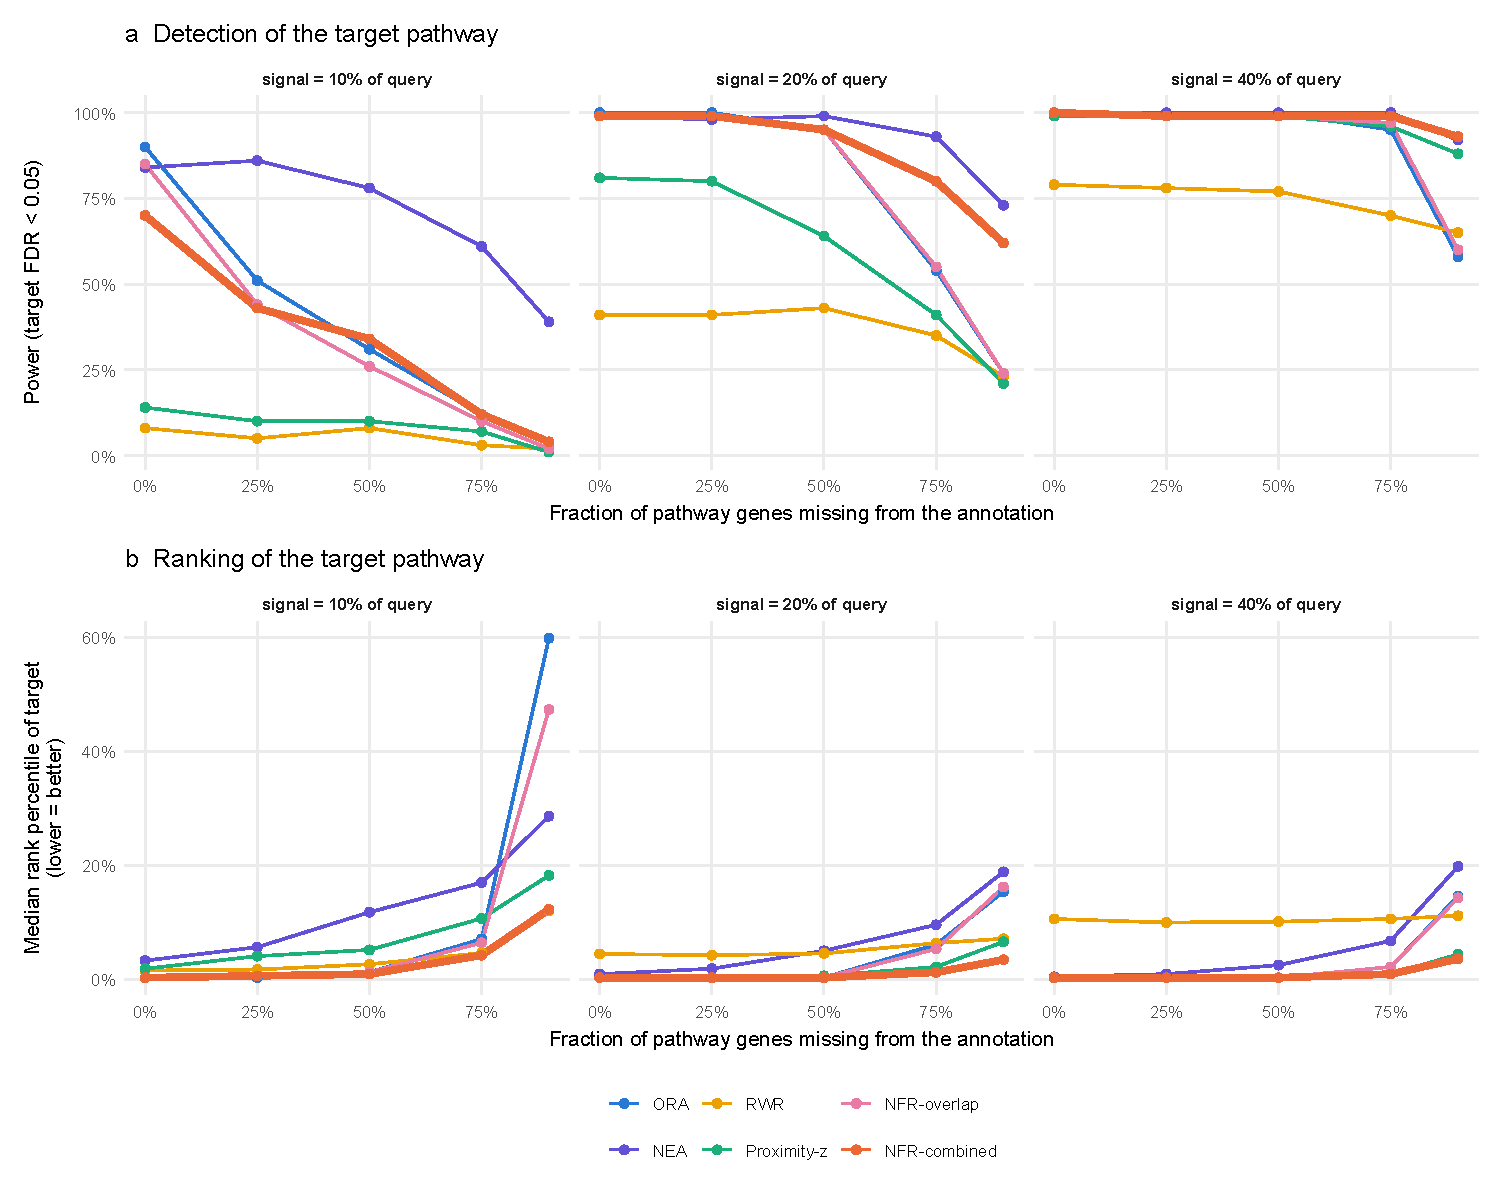
\includegraphics[width=0.95\linewidth]{Fig3_power_incomplete_annotation.pdf}
\caption{\textbf{Power under incomplete annotation.} Query lists of 50 genes contained 10, 20 or 40\% genes from a target KEGG pathway (100 pathways), of which a growing fraction was removed from the tested annotation. \textbf{a} Proportion of simulations in which the target pathway reached FDR $< 0.05$. \textbf{b} Median rank percentile of the target among all pathways. NEA is shown for completeness but is not calibrated (Figure~\ref{fig:calibration}). Single NetFunrankR components are shown in Supplementary Figure~S3.}
\label{fig:power}
\end{figure}

\begin{figure}[p]
\centering
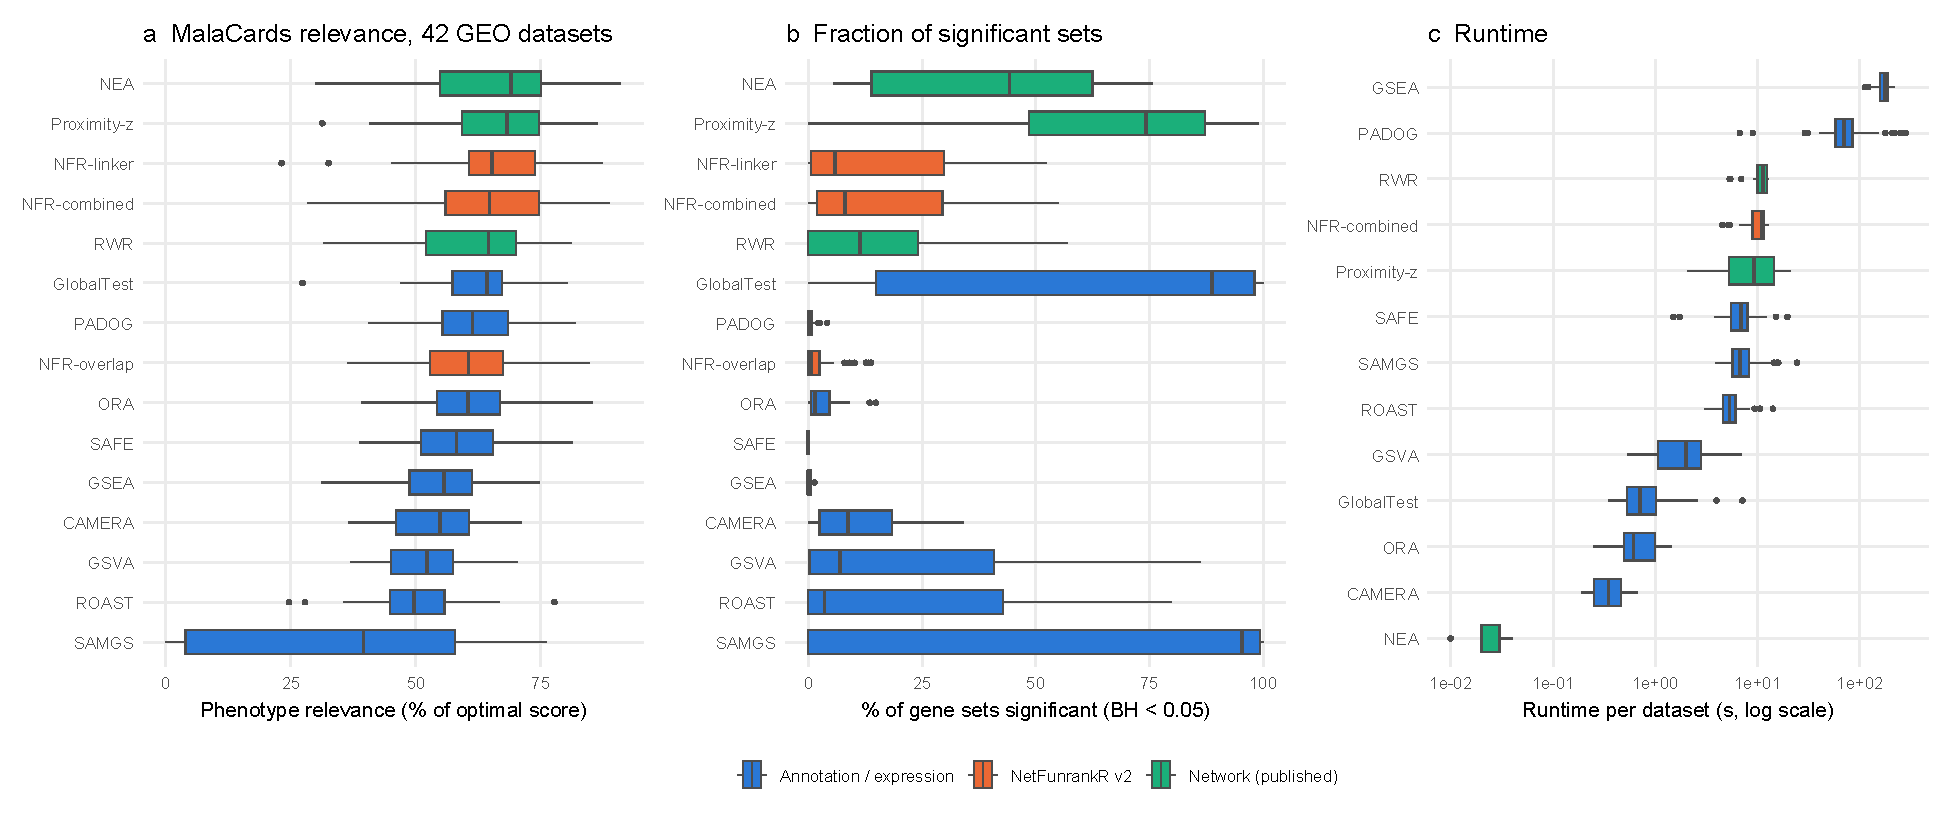
\includegraphics[width=\linewidth]{Fig4_GSEABenchmarkeR.pdf}
\caption{\textbf{GSEABenchmarkeR expression benchmark} (42 GEO datasets, KEGG). \textbf{a} Phenotype relevance of pathway rankings (MalaCards; percentage of the optimal score). \textbf{b} Percentage of gene sets called significant (BH $< 0.05$). \textbf{c} Runtime per dataset. Gene-list methods (ORA, network methods, NetFunrankR) use the differentially expressed genes; the other methods use the full expression data.}
\label{fig:gseabench}
\end{figure}

\begin{figure}[p]
\centering
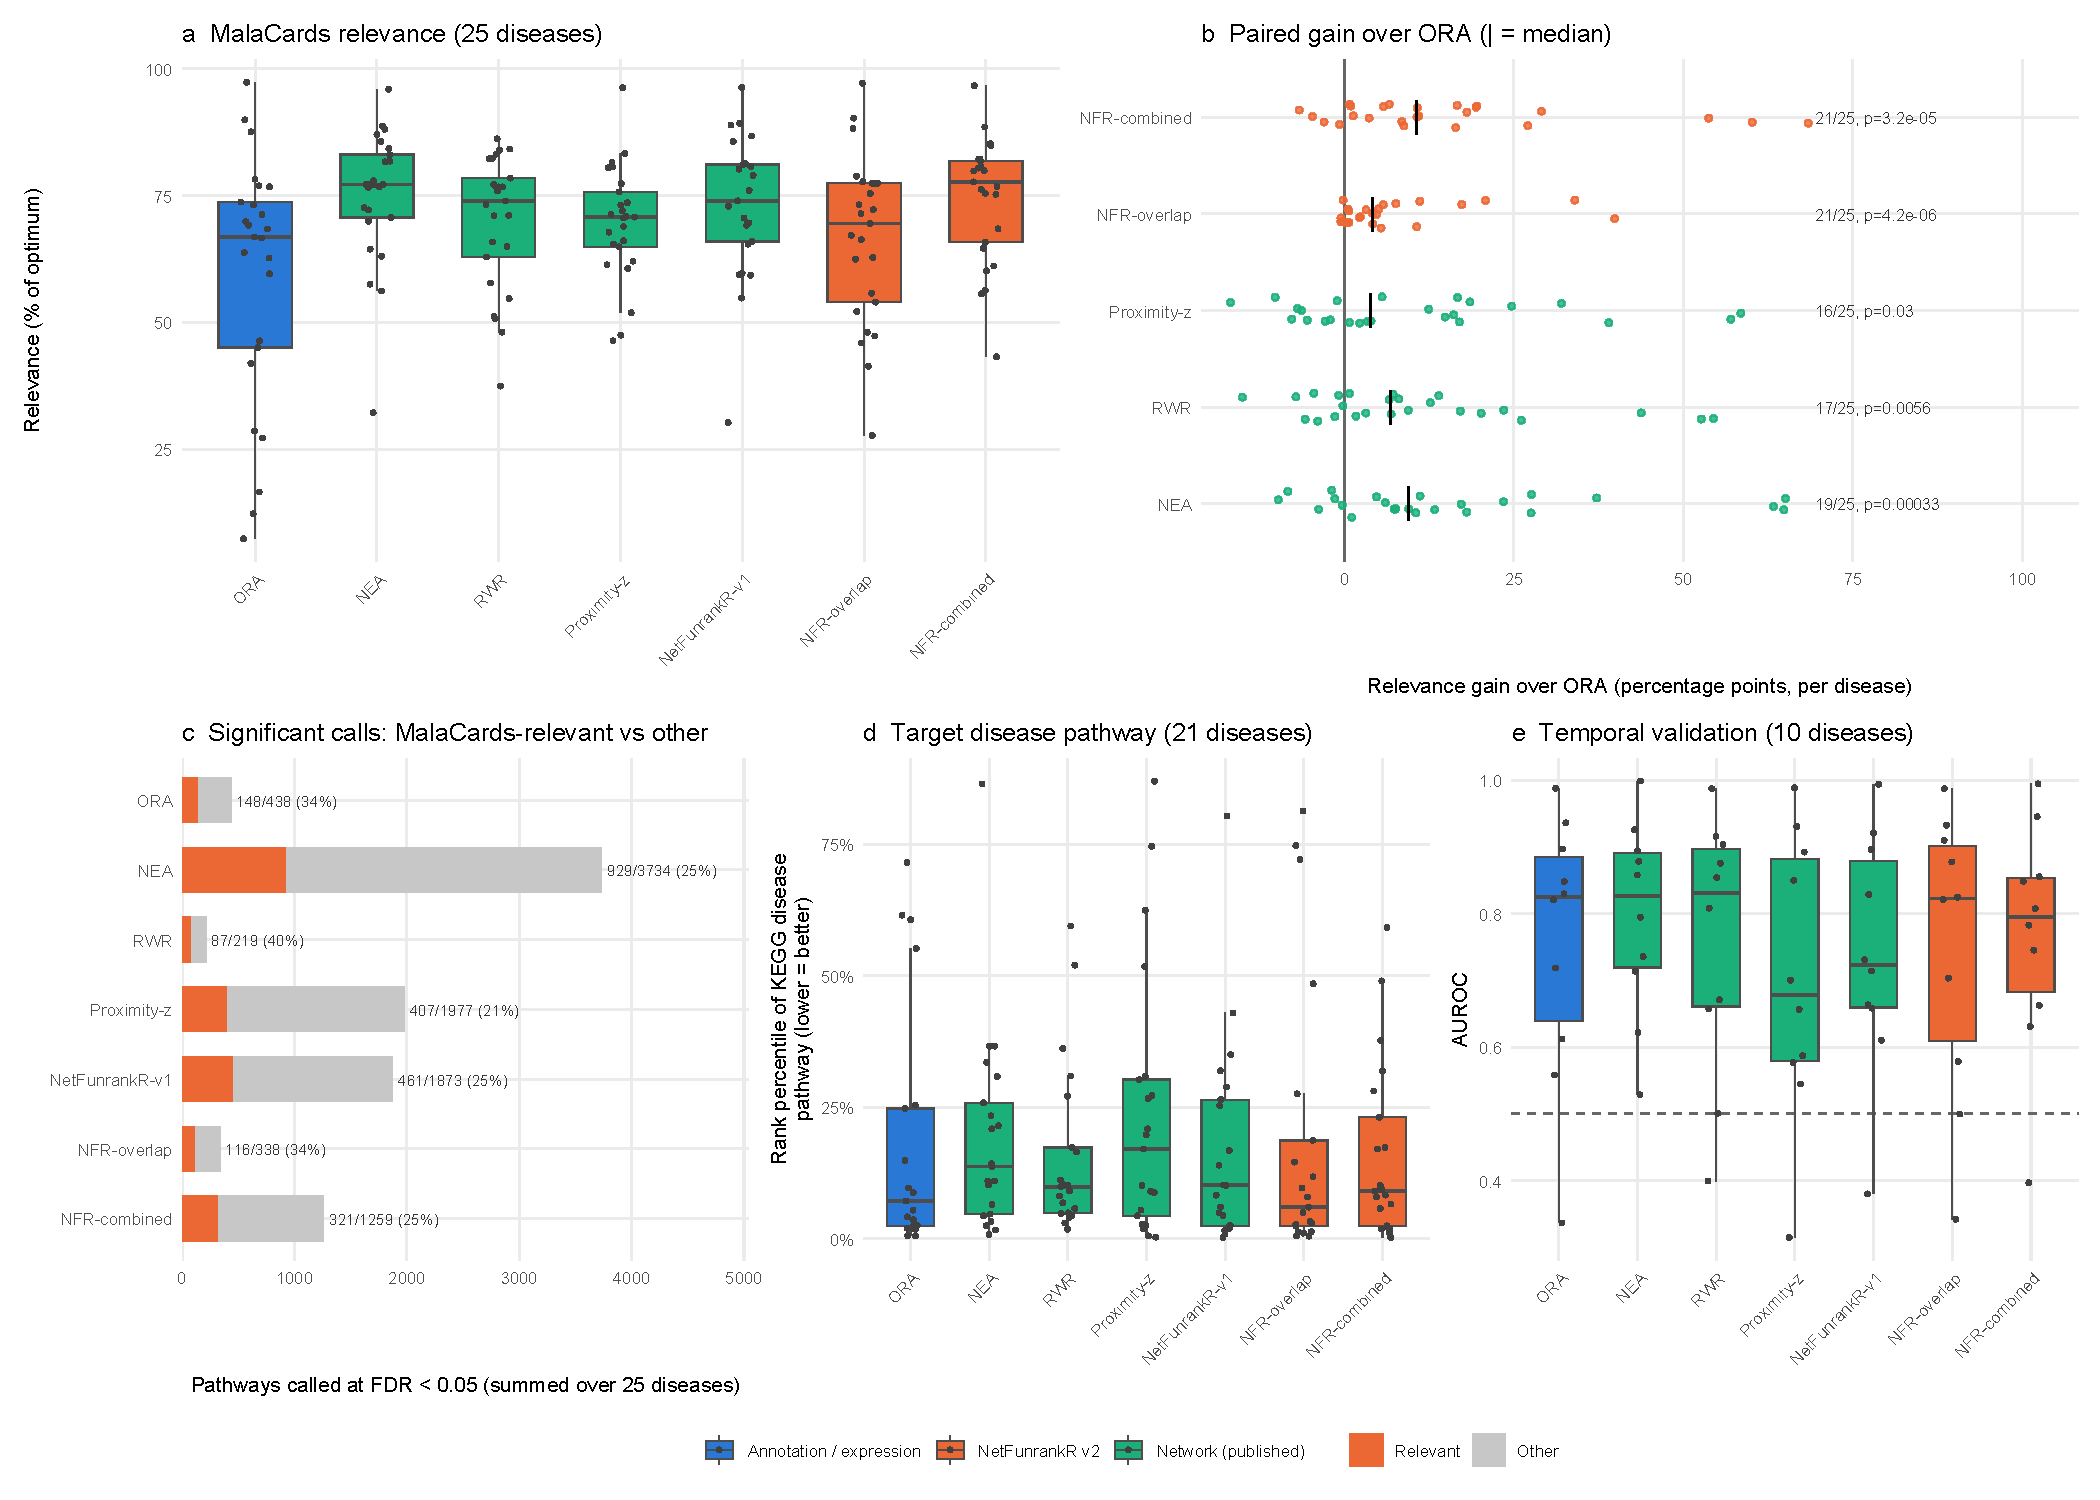
\includegraphics[width=\linewidth]{Fig5_GWAS_benchmark.pdf}
\caption{\textbf{GWAS gene lists of 25 diseases.} \textbf{a} MalaCards relevance of pathway rankings. \textbf{b} Per-disease gain in relevance over ORA (paired Wilcoxon tests; wins/diseases). \textbf{c} Pathways called at FDR $< 0.05$, split into MalaCards-relevant and other pathways (relevant/total and precision). \textbf{d} Rank percentile of the disease's own KEGG disease pathway. \textbf{e} Temporal validation: AUROC of rankings computed from genes reported up to the median discovery date for predicting the pathways over-represented among genes reported later.}
\label{fig:gwas}
\end{figure}

\begin{figure}[p]
\centering
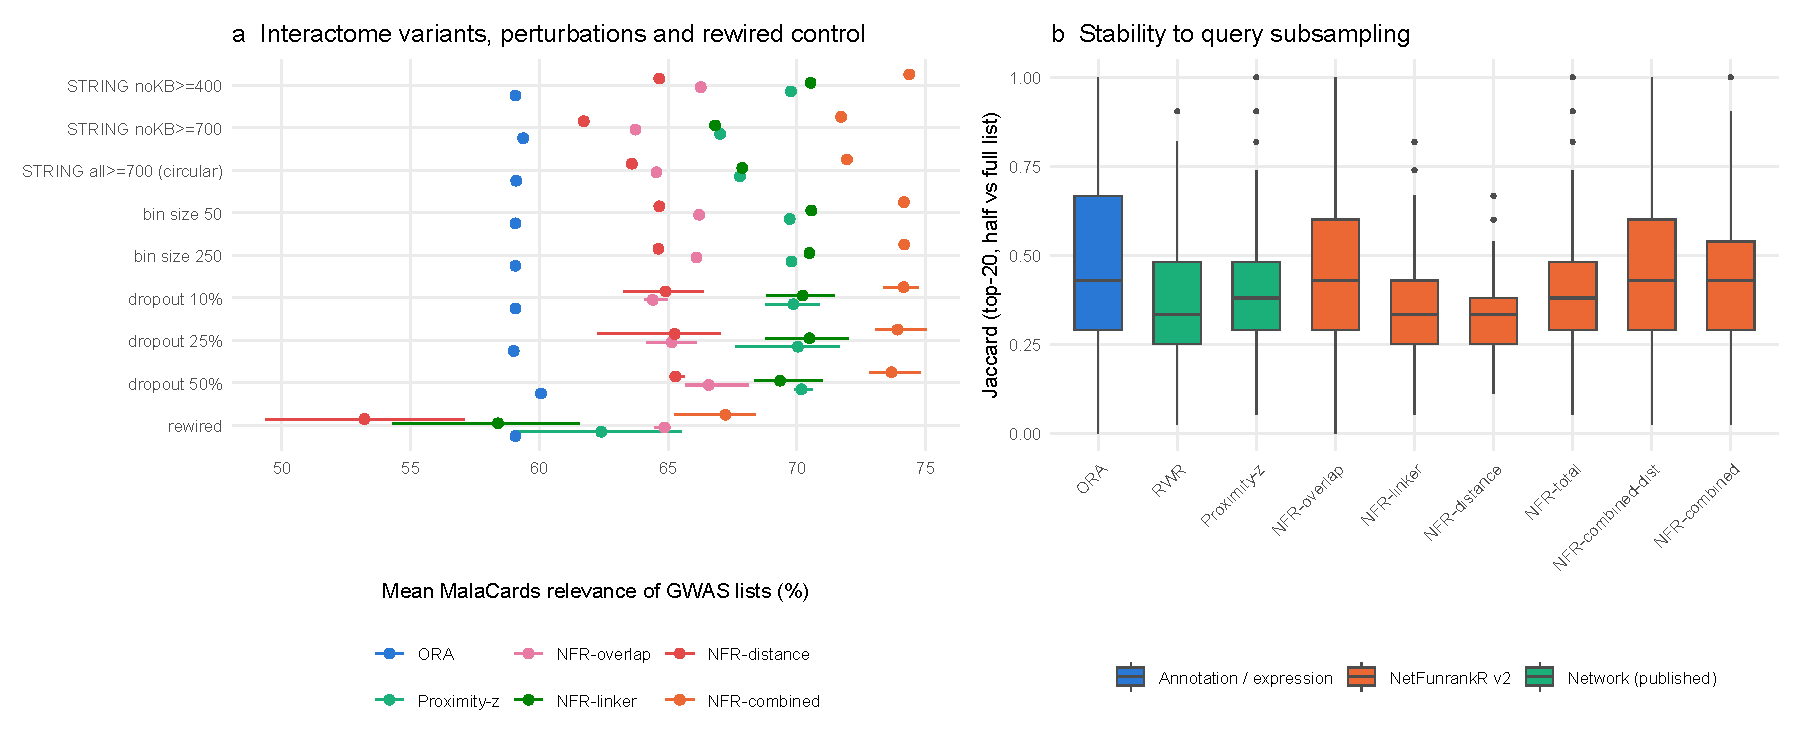
\includegraphics[width=\linewidth]{Fig6_robustness.pdf}
\caption{\textbf{Robustness.} \textbf{a} Mean MalaCards relevance of the GWAS benchmark for alternative interactomes (non-circular STRING at score $\ge$0.4 [default] and $\ge$0.7; full-evidence STRING $\ge$0.7), degree-bin sizes, random removal of edges and degree-preserving rewiring (negative control); bars: range over three replicates. \textbf{b} Jaccard index between the top-20 pathways from random halves of each GWAS list and from the full list.}
\label{fig:robust}
\end{figure}

\begin{figure}[p]
\centering
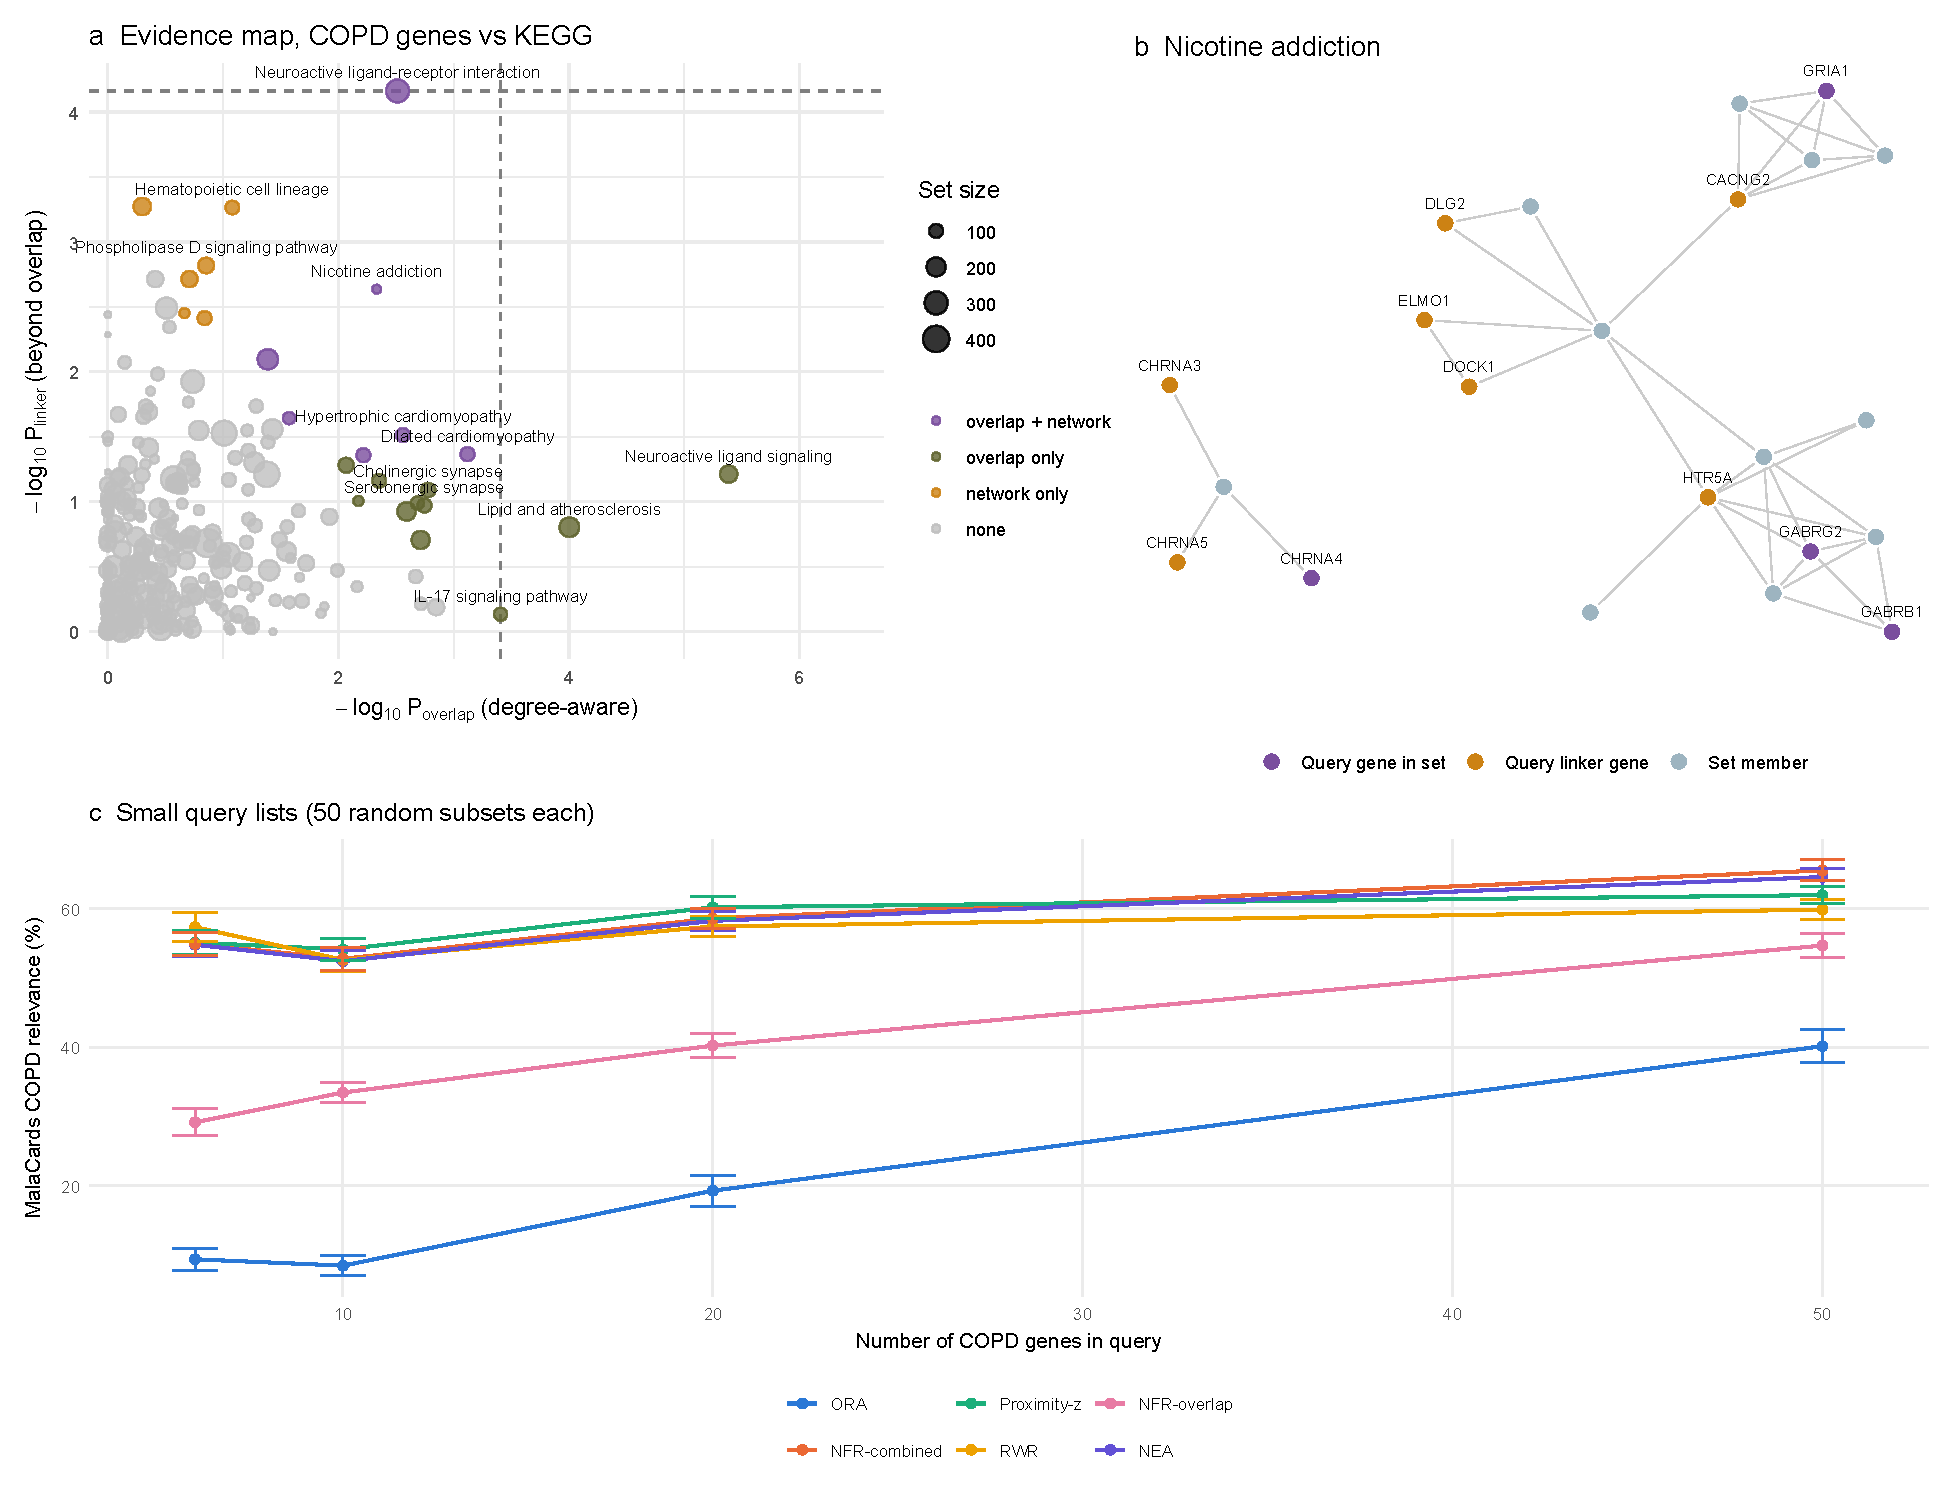
\includegraphics[width=\linewidth]{Fig7_COPD_case.pdf}
\caption{\textbf{COPD case study.} \textbf{a} Evidence map of 363 KEGG pathways for 261 COPD genes: degree-aware overlap evidence versus linker evidence; colours give the evidence class of pathways significant by the combined test (dashed lines: FDR 0.05 thresholds of the single components). \textbf{b} Linker network for \textit{Nicotine addiction}: the 15q25 GWAS genes \textit{CHRNA3} and \textit{CHRNA5}, not annotated to the KEGG pathway, interact directly with its nicotinic-receptor members. \textbf{c} MalaCards COPD relevance obtained from random subsets of 6--50 COPD genes (mean $\pm$ s.e.m., 50 subsets).}
\label{fig:copd}
\end{figure}

\clearpage
\appendix
\section*{Supplementary material}
\renewcommand{\thetable}{S\arabic{table}}
\setcounter{table}{0}
\begin{table}[h]\centering\small
\caption{\textbf{GWAS gene lists.} Genes mapped to genome-wide significant associations ($p\le5\times10^{-8}$) of the GWAS Catalog trait (EFO label pattern), restricted to the interactome; KEGG target disease pathway; temporal split date and numbers of early and late genes (temporal validation used diseases with $\ge$15 genes in both parts and $\ge$3 late-enriched pathways).}
\label{tab:s1}
\begin{tabular}{llrllrr}\toprule
Code & GWAS trait & Genes & KEGG target & Split date & Early & Late\\\midrule
ALZ & Alzheimer disease & 215 & hsa05010 & 2022-04-04 & 120 & 95\\
PARK & Parkinson disease & 157 & hsa05012 & 2019-12-01 & 104 & 53\\
CRC & colorectal cancer & 191 & hsa05210 & 2021-09-30 & 97 & 94\\
BRCA & breast carcinoma & 266 & hsa05224 & 2017-10-23 & 195 & 71\\
PRAD & prostate carcinoma & 396 & hsa05215 & 2021-01-04 & 221 & 175\\
LES & systemic lupus erythematosus & 406 & hsa05322 & 2020-12-03 & 210 & 196\\
DCM & (idiopathic )?dilated cardiomyopathy & 19 & hsa05414 & -- & -- & --\\
PDCO & chronic obstructive pulmonary disease & 357 & -- & -- & -- & --\\
THCA & (differentiated )?thyroid (carcinoma|cancer) & 46 & hsa05216 & -- & -- & --\\
OV & ovarian (serous )?carcinoma & 36 & -- & 2017-03-27 & 20 & 16\\
LAML & acute myeloid leukemia & 561 & hsa05221 & -- & -- & --\\
LGG & glioma & 18 & hsa05214 & -- & -- & --\\
GBM & glioblastoma & 17 & hsa05214 & -- & -- & --\\
PAAD & (exocrine )?pancreatic carcinoma & 30 & hsa05212 & -- & -- & --\\
KIRC & renal cell carcinoma & 73 & hsa05211 & -- & -- & --\\
UCEC & endometrial (carcinoma|cancer) & 15 & hsa05213 & -- & -- & --\\
LUAD & lung adenocarcinoma & 60 & hsa05223 & 2019-07-17 & 34 & 26\\
LUSC & squamous cell lung carcinoma & 46 & hsa05223 & 2017-06-12 & 26 & 20\\
SKCM & (cutaneous )?melanoma & 102 & hsa05218 & 2020-04-27 & 54 & 48\\
STAD & gastric (carcinoma|cancer) & 28 & hsa05226 & -- & -- & --\\
BLCA & urinary bladder (cancer|carcinoma) & 58 & hsa05219 & 2023-05-18 & 30 & 28\\
DMND & type 2 diabetes mellitus & 1387 & hsa04930 & 2020-06-15 & 774 & 613\\
LIHC & hepatocellular carcinoma & 30 & hsa05225 & -- & -- & --\\
TGCT & testicular (germ cell tumor|cancer) & 47 & -- & -- & -- & --\\
CESC & cervical (carcinoma|cancer) & 35 & -- & 2019-09-05 & 18 & 17\\
\bottomrule\end{tabular}\end{table}

\renewcommand{\thefigure}{S\arabic{figure}}
\setcounter{figure}{0}

\begin{figure}[h]
\centering
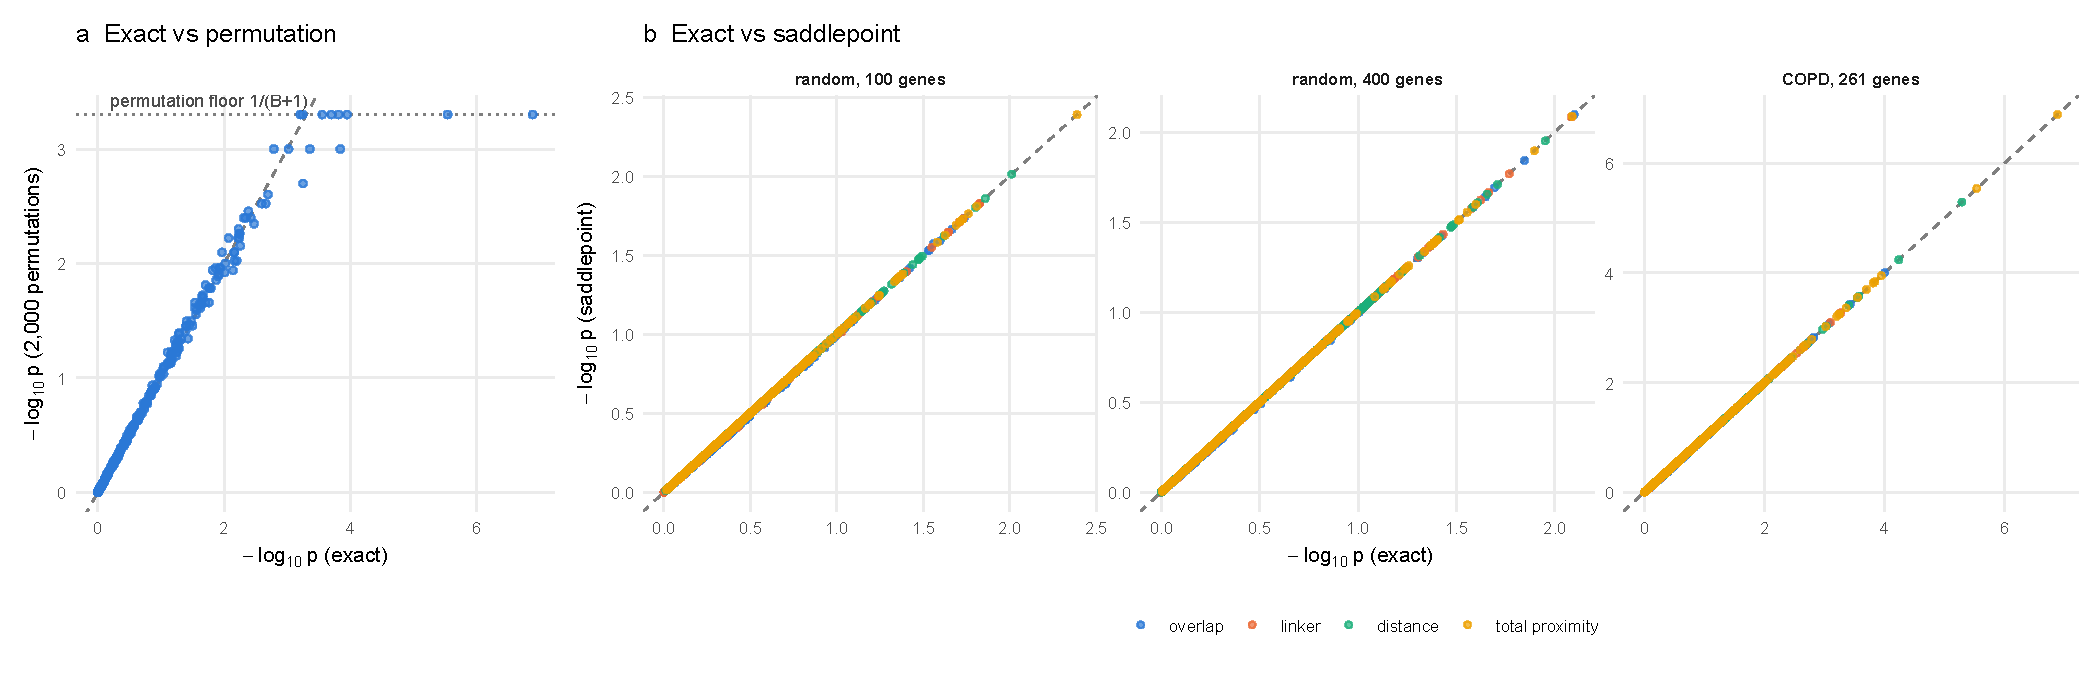
\includegraphics[width=0.9\linewidth]{FigS_null_accuracy.pdf}
\caption{\textbf{Accuracy of the exact and saddlepoint nulls.} \textbf{a} Exact versus Monte-Carlo permutation p-values (2{,}000 permutations) for the total proximity test (COPD genes, KEGG). \textbf{b} Exact versus saddlepoint p-values for hub-biased random lists of 100 and 400 genes and for the COPD list (all tests; maximum absolute difference 0.018 $\log_{10}$ units).}
\label{fig:s_null}
\end{figure}

\begin{figure}[h]
\centering
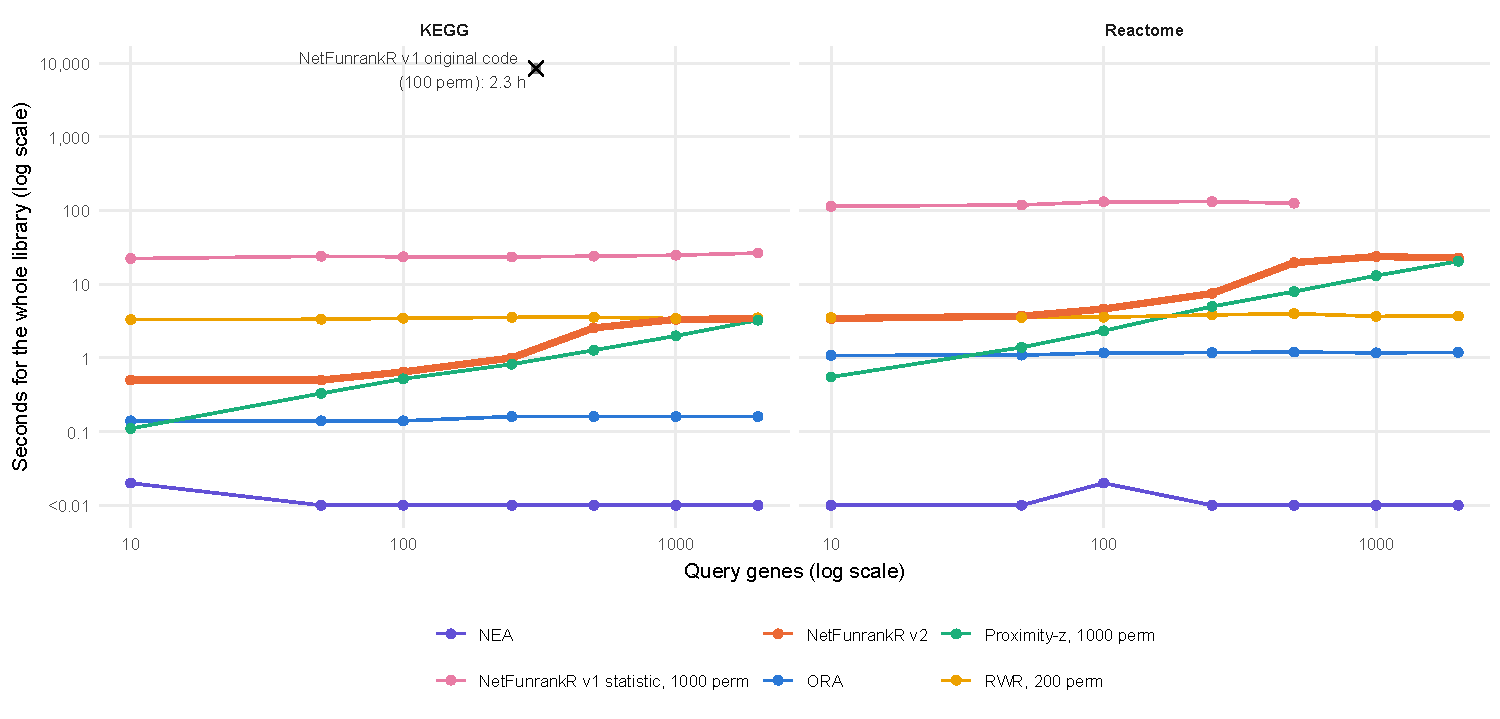
\includegraphics[width=0.9\linewidth]{FigS_runtime.pdf}
\caption{\textbf{Runtime} for a complete library (KEGG, Reactome) on one laptop core, as a function of query size.}
\label{fig:s_runtime}
\end{figure}

\begin{figure}[h]
\centering
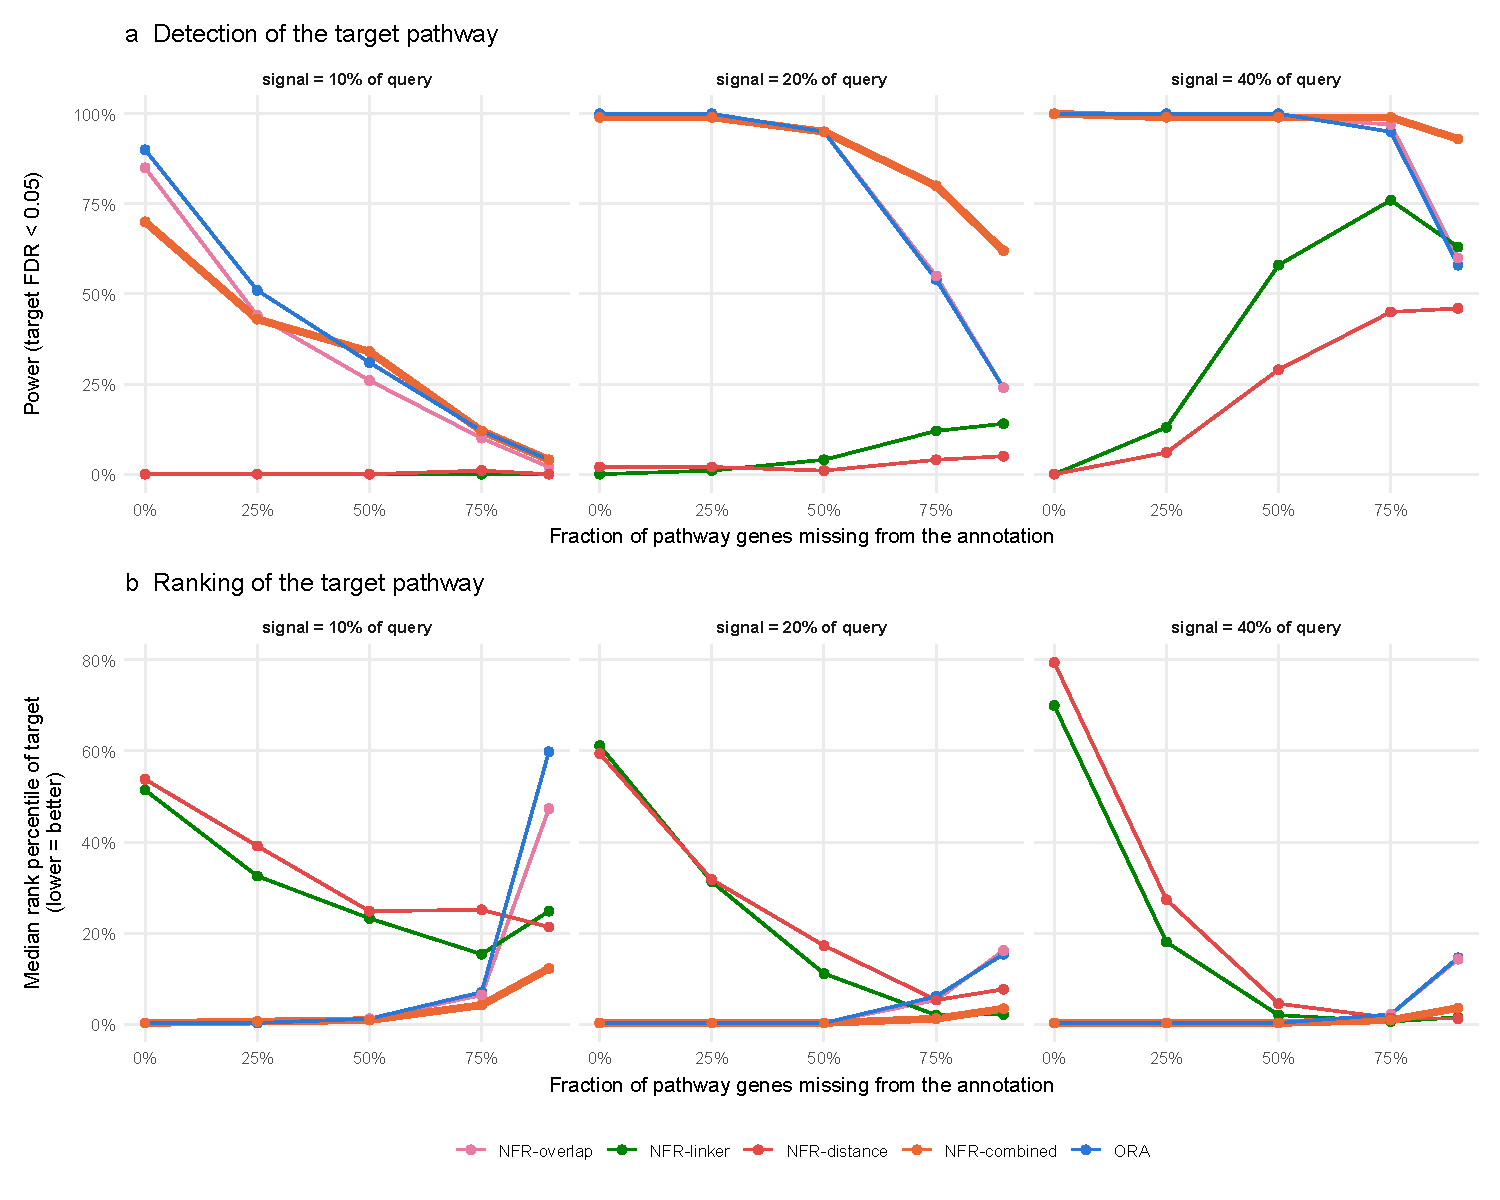
\includegraphics[width=0.9\linewidth]{FigS_power_components.pdf}
\caption{\textbf{Power of the individual NetFunrankR tests} in the incomplete-annotation simulation.}
\label{fig:s_power}
\end{figure}

\begin{figure}[h]
\centering
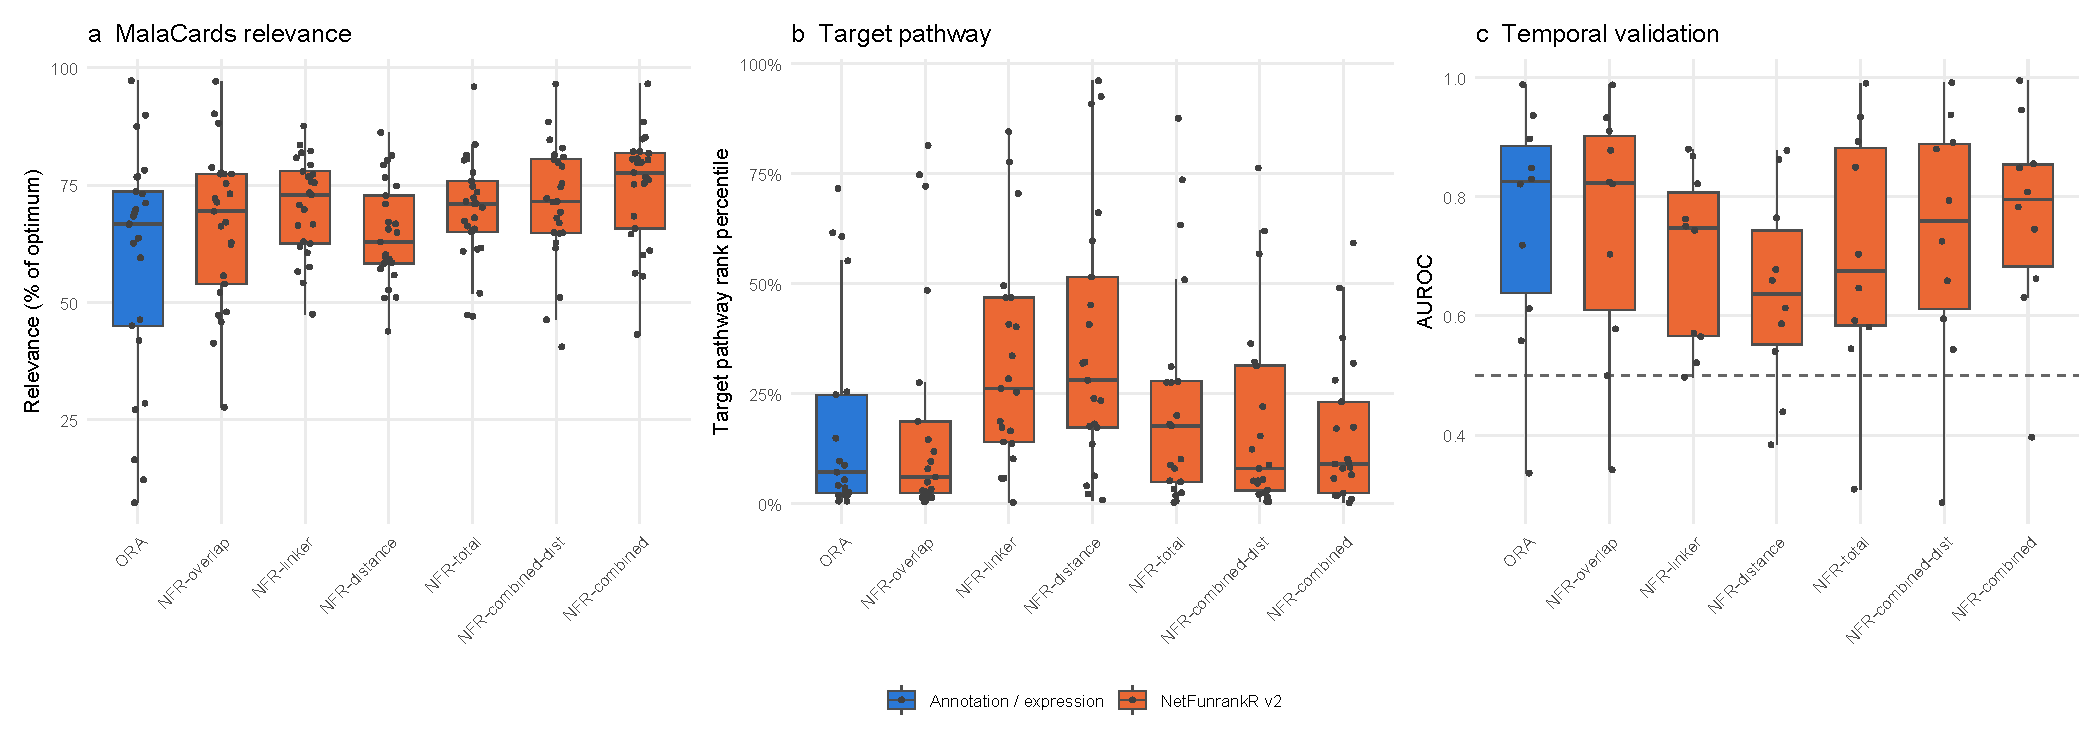
\includegraphics[width=\linewidth]{FigS_GWAS_components.pdf}
\caption{\textbf{Individual NetFunrankR tests on the GWAS benchmark}, including the distance-based combination.}
\label{fig:s_gwas}
\end{figure}

\end{document}
